\documentclass{svjour3} 

% add the option [turnoff] on the following package to remove all notes and todos
\usepackage{amsmath}
%\usepackage[turnoff]{notes}
%\usepackage{notes}
\usepackage{graphicx}
\usepackage{amsfonts}
\usepackage{booktabs}
\usepackage{xspace}
\usepackage{color}
\usepackage{pdfsync}
\usepackage{microtype}
\usepackage{listings}
\usepackage{url}
%\usepackage[draft]{hyperref}
\usepackage{hyperref}
\usepackage{subfig}
\lstset{ %
language=Java,                % choose the language of the code
basicstyle=\small,       % the size of the fonts that are used for the code
%numbers=left,                   % where to put the line-numbers
%numberstyle=\footnotesize,      % the size of the fonts that are used for the
%line-numbers stepnumber=1,                   % the step between two
%line-numbers. If it is 1 each line will be numbered numbersep=5pt,             
% how far the line-numbers are from the code backgroundcolor=\color{white},  % choose the background color. You must add \usepackage{color}
showspaces=false,               % show spaces adding particular underscores
showstringspaces=false,         % underline spaces within strings
showtabs=false,                 % show tabs within strings adding particular underscores
%frame=single,                   % adds a frame around the code
tabsize=2,              % sets default tabsize to 2 spaces
captionpos=b,                   % sets the caption-position to bottom
breaklines=true,        % sets automatic line breaking
breakatwhitespace=false,    % sets if automatic breaks should only happen at whitespace
escapeinside={\%}{)},          % if you want to add a comment within your code
columns=flexible
}
\DeclareCaptionType{copyrightbox}

\pdfminorversion=6

\graphicspath{{figures/}}
\DeclareGraphicsExtensions{.pdf, .png, .ps}

\newcommand{\etal}{\emph{et al.}\xspace}
\newcommand{\paper}[1]{}
\newcommand{\code}[1]{\texttt{#1}}

\newcommand{\todo}[1]{}

\DeclareMathOperator{\typesr}{Types_r}
\DeclareMathOperator{\typesg}{Types_g}
\DeclareMathOperator{\rawtype}{Elide}

% create a hypothesis counter and a command for creating them as well as an autoref name so we can label them and refer back
% to them
\newcounter{hypothesis}
\setcounter{hypothesis}{0}
\newcommand{\hypothesis}[1]{\refstepcounter{hypothesis}\medskip\noindent\textbf{Hypothesis \arabic{hypothesis}} - #1 \medskip}
\newcommand{\hypothesisautorefname}{Hypothesis}

\newcounter{researchQuestion}
\setcounter{researchQuestion}{0}
\newcommand{\researchQuestion}[1]{\refstepcounter{researchQuestion}\medskip\noindent\textbf{Research Question \arabic{researchQuestion}} - #1 \medskip}
\newcommand{\researchQuestionautorefname}{Research Question\xspace}

%for the projects that we talk about in the paper, let's
%define macros for their names so that a) we're consistent
% and b) we can change them easily.

\newcommand{\squirrelsql}{\textsc{Squirrel-SQL}\xspace}
\newcommand{\eclipsecs}{\textsc{Eclipse-cs}\xspace}
\newcommand{\azureus}{\textsc{Azureus}\xspace}
\newcommand{\jedit}{\textsc{JEdit}\xspace}
\newcommand{\spring}{the \textsc{Spring Framework}\xspace}
\newcommand{\junit}{\textsc{JUnit}\xspace}
\newcommand{\maven}{\textsc{Maven}\xspace}
\newcommand{\lucene}{\textsc{Lucene}\xspace}
\newcommand{\jdt}{\textsc{JDT}\xspace}
\newcommand{\hibernate}{\textsc{Hibernate}\xspace}
\newcommand{\commons}{\textsc{Commons Collections}\xspace}
\newcommand{\weka}{\textsc{Weka}\xspace}
\newcommand{\findbugs}{\textsc{FindBugs}\xspace}
\newcommand{\checkstyle}{\textsc{CheckStyle}\xspace}
\newcommand{\logfourj}{\textsc{Log4j}\xspace}
\newcommand{\xerces}{\textsc{Xerces}\xspace}
\newcommand{\ant}{\textsc{Ant}\xspace}
\newcommand{\freemind}{\textsc{FreeMind}\xspace}
\newcommand{\jetty}{\textsc{Jetty}\xspace}
\newcommand{\subclipse}{\textsc{Subclipse}\xspace}

\newcommand{\bbssh}{\textsc{BBSSH}\xspace}
\newcommand{\ehcache}{\textsc{Ehcache}\xspace}
\newcommand{\encuestame}{\textsc{encuestame}\xspace}
\newcommand{\flowgame}{\textsc{flowgame}\xspace}
\newcommand{\hummingbird}{\textsc{Hummingbird}\xspace}
\newcommand{\ice}{\textsc{ice4j}\xspace}
\newcommand{\libgdx}{\textsc{libgdx}\xspace}
\newcommand{\makagiga}{\textsc{Makagiga}\xspace}
\newcommand{\migen}{\textsc{MiGen}\xspace}
\newcommand{\mobac}{\textsc{MOBAC}\xspace}
\newcommand{\pathvisio}{\textsc{PathVisio}\xspace}
\newcommand{\posterita}{\textsc{Posterita}\xspace}
\newcommand{\opensso}{\textsc{OpenSSO}\xspace}
\newcommand{\smslib}{\textsc{SMSLib}\xspace}
\newcommand{\scsreader}{\textsc{SCSReader}\xspace}
\newcommand{\religion}{\textsc{Religion Search}\xspace}
\newcommand{\red}{\textsc{Red5}\xspace}
\newcommand{\vietocr}{\textsc{VietOCR}\xspace}
\newcommand{\xbup}{\textsc{XBUP}\xspace}
\newcommand{\zkdesktop}{\textsc{Zero Kelvin Desktop}\xspace}

\newcommand{\squishlist}{
   \begin{list}{$\bullet$}
    { \setlength{\itemsep}{0pt}      \setlength{\parsep}{3pt}
      \setlength{\topsep}{3pt}       \setlength{\partopsep}{0pt}
      \setlength{\leftmargin}{1.5em} \setlength{\labelwidth}{1em}
      \setlength{\labelsep}{0.5em} } }

\newcommand{\squishend}{
    \end{list}  }


%\makeatletter
%\let\@copyrightspace\relax
%\makeatother


\begin{document}

\pagenumbering{arabic}

\title{Adoption and Use of Java Generics}
%\title{How Do Java Developers Adopt Generics?}
%\title{How Do Java Developers Use Generics?}
%\title{Java Generics Adoption: How New Features are Introduced, Championed, or Ignored}

\journalname{Empirical Software Engineering}

\author{Chris~Parnin,
		Christian Bird,
        and~Emerson~Murphy-Hill}

\institute{C. Parnin \at
              College of Computing, Georgia Institute of Technology, Atlanta, GA, 30332.\\
%               Tel.: +123-45-678910\\
%               Fax: +123-45-678910\\
              \email{chris.parnin@gatech@edu}           %  \\
           \and
           C. Bird \at
              Microsoft Research, Redmond, WA 98052.\\
              \email{cbird@microsoft.com}
           \and
           E. Murphy-Hill \at
              Department of Computer Science, North Carolina State University, Raleigh, NC, 27695.\\
              \email{emerson@csc.ncsu.edu}          	  
}

\date{Received: date / Accepted: date}

\maketitle

\begin{abstract}
Support for generic programming was added to the Java language in 2004,
representing perhaps the most significant change to one of the most widely used
programming languages today. 
Researchers and language designers anticipated this addition would relieve
many long-standing problems plaguing developers, but
surprisingly, no one has yet measured how generics have been adopted and used in practice.
%actually provide such relief.
In this paper, we report on the first empirical investigation into how Java
generics have been integrated into open source software by automatically
mining the history of 40 popular open source Java programs,
traversing more than 650 million lines of code in the process.
We evaluate five hypotheses and research questions about how Java developers use generics.
For example, our results suggest 
that generics sometimes reduce the number of type casts and
that generics are usually adopted by a single champion in a project,
rather than all committers.  We also offer insights into why some features may be adopted sooner 
and others features may be held back.
% These results have several implications for programming language designers
% to consider when designing and deploying new language features.  
% For example, old code may not be patched with new features and migration tools
% may be required.
%example?
\keywords{generics, annotations, Java, languages, post-mortem analysis}
\end{abstract}


\section{Introduction}

Programming languages and tools evolve to match 
industry trends, revolutionary shifts, or refined developer tastes.
But not all evolutions are successes; the technology landscape is pocked with 
examples of evolutionary dead-ends and dead-on-arrival concepts.

Far too often, greatly heralded claims and visions of new language 
features fail to hold or persist in practice.
Discussions of the costs and benefits of language features can easily devolve
into a religious war with both sides armed with little more than 
anecdotes~\cite{markstrum}.
% But this is not so surprising.  Long-gone is the time where it was feasible 
% to re-implement a system in an entirely different programming language.  Even with new language features,
% considerable sea change must occur with developers in the form of education, training, documentation, and processes\,---\,and 
% with programs in the form of migration, redesign, and refactoring old and new code.  
Empirical evidence about the adoption and use of past language features
should inform and encourage a more rational discussion 
% in the future.
when designing language features and considering how they should be deployed.
Collecting this evidence is not just sensible but a responsibility of our community.

In this paper, we examine the adoption and use of generics, which
were introduced as Java version 5 in 2004. 
We take the first look at how features of Java generics,
such as type declarations, type-safe collections, generic methods, and wildcards, have been
introduced and used in real programs.
With the benefit of seven years of hindsight, we investigate how the predictions,
assertions, and claims that were initially made by both research and industry
have played out in the wild.  Further, we investigate the course and timeline of adoption: 
what happens to old code, who buys in, how soon are features adopted, 
and how many projects and people ignore new features?
The results allow us to adjust our expectations about how developers will
adopt future language features.

This paper extends our prior MSR 2011 paper~\cite{parnin11}, where we made
the following contributions:

\squishlist
  \item we enumerate the assumptions and claims made in the past about Java
  		generics (Section~\ref{sec:relatedWork});
  \item	we investigate how 20 open source projects have used\,---\,and
  		have not used\,---\,Java generics (Section~\ref{sec:data} 
  		to~\ref{sec:adoption}); and
  \item we discuss the implications of the adoption and usage patterns of
  		generics (Section~\ref{sec:discussion}).
\squishend

In the prior paper, we examined our research questions and hypotheses from the perspective of \emph{established projects}, projects which started before generics.
This perspective was unique in that it allowed us to observe the impact of a new feature on an existing code base.
In the present paper, we contrast our prior results with the adoption patterns of \emph{recent projects}, projects which started after generics and may offer different perspectives.
Second, we also wanted to compare the adoption of Java generics with an another feature, Java annotations, that were released in conjunction with generics in the Java 5 release.
By examining annotations, an arguably less risky and simpler feature, we have the ability to tease apart some of the factors that influence adoption;
for instance, was Java Virtual Machine compatibility the main barrier to adoption, or was it something else?

%\noindent
In this paper, we add the following new contributions:
\squishlist
  \item we explore 20 new open source projects that were initiated
  		after the introduction of generics and
  \item	we contrast our findings about generics with data on another
  		language feature, Java annotations.
\squishend


\section{Language Feature Overview}

\noindent
%Before describing our investigation of generics in the wild, 
In this section
we briefly describe the motivation and use of Java generics and annotations.
In an effort to maintain consistent terminology, 
we present in \textbf{bold} the terms 
that we use in this paper, drawing from standard terminology 
where possible.
Readers who are familiar with Java generics and annotations may safely
skip this section.

\subsection{Motivation for Generics}\label{sec:lifeWithoutGenerics}

\noindent
In programming languages such as Java, type systems can ensure that certain
kinds of runtime errors do not occur.
For example, consider the following Java code:


\begin{lstlisting}
 List l = getList();
 System.out.println(l.get(10));
\end{lstlisting}

\noindent
This code will print the value of the 10th element of the list.
The type system ensures that whatever object \code{getList()} returns,
it will understand the \code{get} message, and no runtime type error will occur
when invoking that method.
In this way, the type system provides safety guarantees at compile time so that
bugs do not manifest at run time.

Now suppose we want to take the example a step further; suppose that we know
that \code{l} contains objects of type \code{File}, and we would like to know
whether the tenth file in the \code{List} is a directory.
We might naturally (and incorrectly) write:

\begin{lstlisting}
 List l = getList();
 System.out.println(l.get(10).isDirectory());
\end{lstlisting}

\noindent
Unfortunately, this leads to a compile-time error, because
the return type of the \code{get} method is specified at compile-time as 
\code{Object}.
The type checker gives an error because it does not know what types of
objects are actually in the list.

In early Java, programmers had two ways to solve
this problem, the first is casting, and the second we
call \textbf{home-grown data structures}. 
If the programmer implements the casting solution, her code would look like
this:

\begin{lstlisting}
 List l = getList();
 System.out.println(((File)l.get(10)).isDirectory());
\end{lstlisting}

\noindent
The cast is the \code{(File)} part, which forces the
compiler to recognize that the expression \code{l.get(10)} 
actually evaluates to the \code{File} type.
While this solves one problem, it causes another;
suppose that a programmer at some point later forgets 
that the list was intended to hold
\code{File}s, and inadvertently puts a
\code{String} into the \code{List}.
Then when this code is executed, a runtime exception will be thrown 
at the cast.
A related problem is that the code is not as clear as it could
be, because nowhere does the program explicitly specify what kind of objects the list
returned by \code{getList()} contains.
% While we have asserted the programmer \emph{meant} that the list contains
% objects of type \code{List}, the program could also be interpreted such that
% only the 10th element of the list contains a \code{File}.
% This ambiguity exists because the type system does not allow the programmer
% to clearly express her intent.

If the programmer instead implements the home-grown data structure
solution, the code will look like this:

\begin{lstlisting}
 FileList l = getList();
 System.out.println(l.get(10).isDirectory());
\end{lstlisting}

\noindent
Additionally, the programmer would need to create a \code{FileList}
class.
This solution also introduces new problems.
Perhaps the most significant is the code explosion problem; for each and every
list that contains a different type, the programmer will want to create a
different special list class, such as \code{StringList}, \code{IntegerList},
and \code{NodeList}.
These classes will inevitably contain significant duplication, because
they all perform the same functions, differing only by data type.

\subsection{Programming with Generics}\label{sec:progWithGen}

These problems were solved with the 
introduction of \emph{generics} to Java in 2004.
Generics allow programmers to create their own 
\textbf{generic type declarations}~\cite{lesson} 
(we call these \textbf{generic types}, for short).
For example, a programmer can create a 
\textbf{user-defined generic declaration} for a list
like so:

\begin{lstlisting}
 class MyList<T>{
  List internal;
  public T get(int index){
   return (T)internal.get(index);  
  } ...
\end{lstlisting}

\noindent
In this code, the \code{T} is called the 
\textbf{formal type parameter}.
The programmer can use her \code{MyList} class
by instantiating the formal type parameter by using a 
\textbf{type argument}~\cite{lesson},
such as \code{Integer} or \code{File} in the following examples:

\begin{lstlisting}
 MyList<Integer> intList = new MyList<Integer>();
 MyList<File> fileList = new MyList<File>();
\end{lstlisting}

\noindent
Each place where a generic type declaration is invoked (in this example, there are four)
is known as a \textbf{parameterized type}~\cite{tutorial}.
%this particular term is confusing, EMH thinks
On the first line, the programmer has declared the type of the \code{intList} object so that
the compiler knows that it contains objects of type \code{Integer}, and thus that
the expression \code{intList.get(10)} will be of type \code{Integer}.
The result is that the client code is both type safe and clearly expresses the
programmer's intent.
The programmer can also use generic type declarations without taking advantage
of generics by using them as \textbf{raw types}, such as \code{MyList objectList},
in which case the expression \code{objectList.get(10)} will be of type \code{Object}.

In addition to creating their own generic type declarations, programmers can use
generic type declarations from libraries.
For example, software developers at Sun 
\textbf{generified}~\cite{tutorial}, or migrated to use generics, 
the Java collections classes.
For instance, the \code{List} class was parameterized, so that the
previous problem could also be solved like so:

\begin{lstlisting}
 List<File> l = getList();
 System.out.println(l.get(10).isDirectory());
\end{lstlisting}


In addition to using generics in type declarations, 
generics can also be applied to individual methods to
create \textbf{generic methods}, like so:

\begin{lstlisting}
 <A> A head(List<A> l){
  return l.get(0);
 }
\end{lstlisting}

\noindent
In this code, the programmer can pass to the \code{head} method a
generic list containing any type.

\subsection{Motivation for Annotations}

Programmers sometimes want their software to give information
to the tools that run over that software.
For example, a program might want to tell a compiler that a certain
method is deprecated and should no longer be called~\cite{annotation_guide} or a class
might want to tell its environment that it represents a web service~\cite{annotation_interview}.
Prior to Java 5, such mechanisms to communicate with 
tools were \emph{ad hoc}.
For example, before Java 5, 
the \code{\@Deprecated} tag in a JavaDoc comment
indicates whether a method is deprecated,
while an external descriptor file indicates that a class is web service.

\subsection{Programming with Annotations}

With Java 5, the annotation language feature was introduced as a unified
syntax for programs to issue directives to tools.
To use an annotation, the programmer puts an @ symbol followed by an annotation
name just before a program element (such as a class or method), 
and, if the annotation has values, sets those values in curly brackets.
For instance, to tell the compiler that the \code{head} method is deprecated, the programmer
can write the following:

\begin{lstlisting}
 @Deprecated
 <A> A head(List<A> l){
\end{lstlisting}

\noindent
When a program is compiled, the compiler warns the programmer about any code that 
references this method.
If the programmer wants to mark a class as a web service, she can write the following:

\begin{lstlisting}
 @WebService
 public class MyWebService{
\end{lstlisting}

The \code{@Deprecated} annotation is an example of an annotation recognized by the Java
5 compiler. Two other annotations are recognized by default by the compiler: the \code{@Override} annotation,
used for indicating that a method overrides a method in a superclass,
and the \code{@SuppressWarnings} annotation, used for telling the compiler not to 
generate certain warnings when compiling~\cite{annotation_tutorial}.
The \code{@WebService} annotation is an example of an annotation defined in a specific
API.  Often these types of annotations are discovered and inspected via reflection and
used for purposes such as automatically generating wrapper code or configuring framework properties.
Users can define their own custom annotations as well, although a discussion
of how this is done is beyond the scope of this paper.
%maybe want to talk about this more if we see some examples in the projects

\section{Related Work}\label{sec:relatedWork}
 
%Enumerate the things people claim/assume about generics.
%Talk about the nearest empirical studies and how they are 
%inadequate.
%\note[Bird]{Below is taken from my earlier literature and is still a little rough}

\noindent
In this section, we discuss previous claims about and studies of generics.

\subsection{Claims Regarding Generics}

When Sun introduced generics, they claimed that the language feature was ``a
long-awaited enhancement to the type system'' that ``eliminates the drudgery of
casting.''
Sun recommended that programmers ``should use generics everywhere [they] can.
The extra efforts in generifying code is well worth the gains in clarity and type
safety.''\footnote{\scriptsize{\url{http://download.oracle.com/javase/1.5.0/docs/guide/language/generics.html}}}

\noindent
There have been a number of papers and books that have extolled
the benefits of using generics in several contexts.
We list here a sample of such claims.

In \textit{Effective Java}, Bloch~\cite{bloch2008ej} asserts that
when a programmer uses non-generic collections, she will not discover errors 
until run time.  
Even worse, the error is manifest as a \code{ClassCastException} when taking an item
\emph{out} of a collection, yet to correct the error,
she must time-consumingly identify which object was wrongly inserted \emph{into} the collection. 
By using generics, the type system shows the developer exactly where she inserted the 
incorrect object, reducing the time to fix the problem.
%Further, she will no longer have to manually cast elements when
%retrieving them from collections.

In their paper on automatically converting Java programs to
use generic libraries, Donavan~\etal~\cite{donovan2004cjp} assert:

\squishlist
\item In pre-generic Java, programmers thought of some classes in pseudo-generic
terms and tried to use them in such a way.  However, without a generic
type system, they would make inadvertent errors that would show up at
runtime.  The addition of generics to the type system moves these runtime
errors to compile time type errors.

\item The type system represents an explicit specification, and 
generics strengthen this specification.
This is better for developers because they can use this strong specification to reason about
the program better and are less likely to make mistakes.  
In addition, the compiler can enforce the specification.

\item Prior to generics, programmers that wanted type safe containers would write
their own home-grown data structures, increasing the amount of work
and likelihood of error, compared to using data structures in libraries.
% Sometimes these were simply wrappers around
% existing collections classes and sometimes they were home-grown data structures.
%Both approaches mean additional work and also increased likelihood of error.
Such structures also ``introduce
nonstandard and sometimes inconsistent abstractions that require
extra effort for programmers to understand.''
\squishend

In his book on C++ templates, Vandevoorde \cite{vandevoorde2003c++} asserts
that when the same operations need to be performed on different types, 
the programmer can implement the same behavior repeatedly for each type.
However, if in doing so she writes and maintains many copies of similar code, she will make
mistakes and tend to avoid complicated but better algorithms because they are
more error prone.  
She must also deal with all of the difficulties
associated with code clones such as making orchestrated changes to coupled
clones~\cite{geiger2006rcc} and perform maintenance more frequently~\cite{monden2002software}.

%In 2004, Sun released a tutorial for generics~\cite{bracha2004generics}, which makes the following claims 
%about the use of generics:
%\note[Emerson]{This list much like the list in the intro: remove duplication}

%\begin{enumerate}
%\item abstract data structures over types
%\item removes casts, and thus runtime errors become compiletime errors
%\item Programmers can express their intent more explicitly, to the compiler \emph{and} the programmer
%\item ``improved readability and robustness''
%\item Generic methods allow common functionality to apply to generic types.
%\end{enumerate}

Naftalin and Wadler~\cite{naftalin2006Java} claim that generics 
work ``synergistically'' with other features
of Java such as \emph{for-each} for loops and autoboxing.  
They also claim that there are now fewer details for the programmer to remember.  
They also claim that generics can make design patterns more flexible by
presenting an example of a
visitor pattern that works on a tree with generic elements.
%and an interpreter which works on generic types.  

In summary, the claims made by previous authors are:

\squishlist

\item Generics move runtime errors to compile time errors. % donovan2004cjp
%\item Generics give a \emph{guarantee} that certain runtime type errors will not occur. % bloch2008ej
\item Programmers no longer have to manually cast elements from pseudo-generic data structures or methods. % bloch2008ej

\item Typed data collections such as \code{FileList}, create non-standard and sometimes inconsistent abstractions. % donovan2004cjp
\item Generics prevent code duplication and errors resulting from maintaining multiple typed data collections. % vandevoorde2003c++

\item Generics enhance readability and specification. % donovan2004cjp
\item Generics lower cognitive load by requiring the programmer to 
remember fewer details. % naftalin2006Java
\squishend

\subsection{Empirical Studies of Generics}

\noindent
There have been few empirical studies related to the use of generics in Java or
parameterized types in object oriented languages in general.  Here we discuss
the few that exist.

In 2005, Basit~\etal~\cite{basit2005empirical} performed two case studies
examining how well generics in Java and templates in C++ allowed what they
termed ``clone unification.'' They found that 68\% of the code in the Java
Buffer library is duplicate and tried to reduce these clones through
generification.  About 40\% of the duplicate code could be
removed.  They observed that type variation triggered many other non-type
parametric differences among similar classes, hindering applications of
generics.  They also observed heavy cloning in the C++ Standard Template Library as well.

Fuhrer~\etal~\cite{fuhrer2005efficiently} implemented refactoring tools 
that would replace raw references to standard library classes with
parameterized types.
In evaluating the refactoring tools on several Java
programs, they were able to remove 48.6\% of the casts and 91.2\% of the
compiler warnings.

We are not the first to examine how well features intended to aid programmers
live up to their claims.  Pankratius \etal performed an empirical study aimed
at determining if transactional memory actually helped programmers write
concurrent code~\cite{pankratius2009does}.  They found some evidence
that transactional memory (TM) did help; students using TM completed
their programs much faster.  However, they also spent a large amount of time
tuning performance since TM performance was hard to predict.  
%Although a completely different topic, we differ from Pankratius's work in that we
%examine \emph{existing} software rather than perform a study where students
%create software from scratch using different language features.

These studies differ from our study in that they investigated generics or another language feature 
in an artificial or laboratory context, whereas we investigate generics in several natural
contexts: open source software. As a result, these studies investigate the ideal impact of generics,
while our study investigates their real impact.

\subsection{Empirical Studies of Annotations}

In this paper we contrast the adoption of Java generics with adoption
of Java annotations.
While many researchers have introduced new types of annotations, such
as for extended type checking~\cite{flanagan} 
and pluggable types~\cite{papi},
little work has studied the use of annotations in existing programs.
The most relevant empirical research that we know 
of is Shi and colleagues' study of how API documentation 
changes over time~\cite{shi}.
Specifically, the authors looked at how Java API annotations are changed in
five real-world libraries in order to understand
how API documentation evolves.
In contrast, the study presented in this paper
analyzes a wider variety of Java annotations
in order to understand how language features are adopted.

Other research has investigated how annotation-like source
code constructs are used.
For example, Liebig and colleagues studied the use of C
preprocessor directives to understand whether those
directives align with the source code they accompany~\cite{liebig}.
As another example, Storey and colleagues studied how developers
tag their code with task markers (such as ``TODO'')
to understand how developers manage tasks~\cite{storey}.
In contrast to these studies, the current papers seeks to 
study the use of annotations as a means to understand 
language feature adoption.

% other annotations paper
% 	-http://dl.acm.org/citation.cfm?id=378831
% 	-http://dl.acm.org/citation.cfm?id=1390656 (pluggable types)

\section{Investigation}\label{sec:investigation}

Our investigation begins with understanding how developers use generics in
programs.
Are some features of generics widely used and others never touched?
Next, we examine claims made about generics and see if the purported benefits of generics are realized in practice.
Finally, how does adoption play out\,---\,how soon does it occur, what happens to the old code, who buys in?


We start with a data characterization by measuring how widespread generics are
among our selected projects and their developers.  Then, we examine in detail
how that usage varies across the features of generics.

%We measure the following features of generics: 
%declarations, instantiations,
%user-defined generic methods and classes, 
%parameterizations, wildcards.

%\subsection{Hypotheses}
\subsection{Investigated Claims}

%Rather than an open-ended investigation into how developers use Java
%generics, we focused our investigation by reviewing prior literature 
%for prior claims that researchers have made about generics.
%In this section, we formulate prior claims about generics in the form
%of hypotheses, which we will evaluate in Section~\ref{sec:results}.

%Donovan \textit{et al.}~\cite{donovan2004cjp} have asserted that developers
%desire type-safe containers.
%Prior to version 5, Java already had a rich collections library
%which often obviated the need of developers to write their own.  
%Based on our own experience, discussions with OSS developers, 
%and the focus of prior work on 
%collections~\cite{fuhrer2005efficiently}, we expect
%that the majority of generic use will be limited to 
%the standard Java generics collections:
%
%\hypothesis{The majority of generic use will be utilizing 
%collections from the Java standard library.}
%\label{hypo:standard_collections}

One of the claims regarding generics (identified previously)
is that they reduce the number of runtime exceptions~\cite{bloch2008ej}.
Ideally, we would like to know how many \code{ClassCastException}s
a program threw before generics were introduced,
then compare that to the number thrown after generics were introduced.
If the claim is true, the number of thrown
\code{ClassCastException}s should be reduced.
To investigate the feasibility of this type of analysis,
we manually searched the bug repositories of three
large projects (\jdt, \spring, and \opensso) for
valid bug reports containing \code{ClassCastException}s.
Overall, we found very few bug reports 
regarding \code{ClassCastException}s: 
in \jdt, only about 10 \code{ClassCastException} bugs were reported per year;
in \spring, only about 13 per year,
and in \opensso, only about 5 per year.
%opensso -> 27 issues, dec06->jan12, 27/6 = 5 per year
%spring  ->150 issues, mar04->jan12, 103/8 = 13 per year
%jdt     ->431 issues, 10/01->1/12 ->126/11 = 10 per year
In smaller projects, the number of reported \code{ClassCastException}s
is likely much smaller.
We hypothesize that the problem is not so much that \code{ClassCastException}s
occur infrequently, but that they are usually introduced and fixed
before the software is released.
Because of the low number of bug reports about \code{ClassCastException}s,
we reasoned that this was not a feasible approach to perform a temporal,
statistical analysis to investigate the
claim about generics reducing runtime exceptions.
We also rule out dynamic approaches where we would run each
version of a program due to the state space explosion problem, 
which is compounded by the thousands of different versions of many open source
projects.

%Instead, we restate the problem as how the number of casts
%in a program changes over time.
%Although a cast is not the same as a runtime exception,
%we reason that each cast represents
%a non-zero probability that a runtime exception will occur.
However, Bloch, in his remarks about runtime exception, continues with a related claim that 
casts would also be reduced by the introduction of generics~\cite{bloch2008ej}.  
Researchers consider casts to be a code smell~\cite{Emden2002Detect}, indicating poor code structure and a catalyst for runtime exceptions.
We reason that evidence of reducing casts also gives evidence of reducing probability of runtime exceptions by a non-zero amount.
Thus, we investigate:

\hypothesis{When generics are introduced into a codebase, 
the number of type casts in that codebase will be reduced.}
\label{hypo:cast_reduction}

%Parnin and Bird observed that intro of generics
% tends to make the casts ``flatline'' in the codebase.  
% ``It stops the cancer''

\noindent

%We also investigated the claim of code reduction. Specifically, the claim was that without generics, 
%developers would have to manually duplicate and parameterize type-specific containers for user-defined container classes. But with generics,
%developers would prevent this duplication from occurring.
%Therefore, we looked at whether this claim was based on a realistic premise; could have developers simply maintained a small set of 
%duplicated container classes or would there be an unreasonable explosion of container types, thus necessitating the introduction of generics.

We also investigated Donavan's claim that without a mechanism such as generics, it would be necessary for programmers to introduce code duplication in order to achieve type safety. Donavan argued that developers would be forced to create data structures for every type of data they wanted to store.  If we assume that Donavan's claim is valid, then we can measure the worse-case cost for achieving type-safety via the method proposed by Donavan. Specially, we can estimate the amount of duplication and bugs that would arise from having to maintain the duplicated type-safe version of classes.  There are several reasons why this is an worse-case estimate: \emph{e.g.,} developers may find ways to factor out commonalities in non-type safe code.  But, taken more generally, these measures provide a simple way of quantifying the value of generics by observing if types are instantiated with more than one parameter.

%\hypothesis{Introduction of user-defined generics classes reduce code-duplication.}
%\hypothesis{Introduction of user-defined generics classes was necessary for preventing duplication of many cloned container classes.}
\hypothesis{Manually maintaining type-safe code would be costly due to maintaining a high number of clones.}

\label{hypo:codedup_reduction}

\subsection{Adoption Research Questions}

Although a wealth of prior literature has examined how open source software (OSS)
projects make decisions, assign and accomplish tasks, and organize themselves 
(e.g.~\cite{ducheneaut2005sos,mockus2002two,omahony2007emergence}), 
the nature of adoption of new language features such as Java generics or annotations is not clear.

Our first research question investigates if there will 
be a concerted effort to convert old code to use the new generic language feature.  
Are the new features compelling enough to fix old 
code that may contain problems that would be fixed by generics 
or at least to maintain consistency?
In other words:

\researchQuestion{Will there be large-scale efforts to convert old code using raw types to use generics?}
\label{hypo:migration}


Our second research question centers around how project members embrace new language 
features such as Java generics and annotations.
Do they do it together, or do some members still hold out?  
Even though ``benevolent dictatorships'' exist in OSS, nearly every open source project's 
decision-making process is governed in at least a semi-democratic fashion.

Since the decision to use a new feature has implications directly
on the codebase itself (e.g., it may require using a newer JDK
or modify popular method signatures impacting all call sites),
we expect that there will be project-wide acceptance
of new features rather than acceptance by individual members.
We would also expect our research question to have consistent answers for both generics and annotations:

% Parnin>Bird: I like this text, but it's just too long for the space we have!

%Even though ``benevolant dictatorships'' exist in OSS,
%\footnote{Python lead by
%Guido Van Rossum as a benevolent dictator, but large decisions are always
%weighed in on by the community.} 
%nearly every open source project's decision
%making process is governed in at least a semi-democratic fashion.
%For example, in the Apache project, there is a core board that makes decisions~\cite{apache_foundation} and
%in the Python community, there is often broad discussion regarding
%important decisions~\cite{ducheneaut2005sos} and informal voting regularly occurs~\cite{python_voting}.
%The need for a democratic process is clear;
%the lack of following such a process has led to, in cases such as XFree86, forking and
%disbandment.  
%Since the decision to use generics has implications directly
%on the codebase itself \todo[Bird]{give an example of an implication},
%we expect that there will be project-wide acceptance
%of generics rather than acceptance by individual members:
% or in individual subsystems:

%\todo[Chris]{Move these hypothesis to Research Questions, because we want to know how much,
%not just if a hypo is supported based on an arbitrary threshold.}

%\hypothesis{There will be broad use of generics by project members once generics are introduced into a project.}
\researchQuestion{Will project members broadly use new language features after introduction into the project?}
\label{hypo:community_acceptance}

Finally, Java integrated development environments (IDEs) such as Eclipse, Netbeans, and IntelliJ IDEA all 
support features such as syntax highlighting and semantic analysis to provide auto completion
and identify type errors interactively.  These tools enable developers to be more productive, 
but not all IDEs supported generics when they were first introduced.  Additionally, developers are often constrained by 
the platforms they are intended to deploy on. We expect that the 
choice to use new language features such as generics or annotations will in part depend on the tool support
available and platform support for those features.

\researchQuestion{What factors influence adoption of new language features?}
\label{hypo:ides}

\subsection{Projects Studied}

To test our hypotheses and evaluate our research questions, 
we automatically analyzed 40 open source software projects.

For the first 20, we analyzed 
the top ``most used'' projects according to \url{ohloh.net}, selecting only
projects with significant amounts of Java code.
We chose to select projects from \url{ohloh.net} because the site contains the most comprehensive
list of open source projects of which we are aware.
The 20 selected projects can be seen in~\autoref{table:20establishedprojects}. 
%\ant, 
%\azureus, 
%\checkstyle, 
%\commons, 
%\freemind, 
%\findbugs, 
%\jetty, 
%\jedit, 
%\jdt,
%\junit, 
%\eclipsecs, 
%\hibernate, 
%\logfourj, 
%\lucene, 
%\maven, 
%\spring, 
%\squirrelsql, 
%\subclipse, 
%\weka, 
%and
%\xerces.

%%%%%%%%%%%%%%%%%%%%%%%%%
%%%Table 20 established projects
\begin{table*}[ht]

\begin{center}
%\begin{tabular*}{17.75cm}{@{\extracolsep{\fill}}|p{0.15cm}|p{2cm}|p{1.5cm}|p{0.5cm}|r|r|r|r|r|r|r|}
\begin{tabular*}{12.5cm}{@{\extracolsep{\fill}}p{4cm}rrrrrrr}

\textbf{Project Name} &\textbf{Devs}&\textbf{Age}&\textbf{Start}&\textbf{End}&	 \textbf{LOC} \\
\hline\\
\ant	         							&	38		&	10	&	1/13/2000 	&	11/15/2010 	&		85,736	\\[1mm]
\azureus	    							&	29		&	6		&	7/7/2003 		&	4/01/2010 	&		130,440	\\[1mm]
\checkstyle									&	5			&	6		&	6/22/2001 	&	12/13/2007 	&		174,611	\\[1mm]
\commons 										&	27		&	9		&	4/14/2001 	&	10/22/2010 	&		235,487	\\[1mm]
\eclipsecs									&	6			&	7		&	5/21/2003 	&	6/30/2010 	&		592,214	\\[1mm]
\textsc{Eclipse-JDT} (\jdt)	&	69		&	9		&	5/2/2001		&	11/19/2010 	&		45,979	\\[1mm]
\findbugs										&	29		&	7		&	3/24/2003 	&	10/25/2010 	&		27,894	\\[1mm]
\freemind										&	4			&	8		&	8/1/2000 		&	7/17/2009 	&		175,042	\\[1mm]
\hibernate									&	23		&	4		&	11/29/2001 	&	2/27/2006		&		3,125,097	\\[1mm]
\jedit											&	94		&	10	&	1/16/2000 	&	6/30/2010 	&		52,031	\\[1mm]
\jetty											&	13		&	10	&	8/6/1998 		&	5/15/2009 	&		90,862	\\[1mm]
\junit											&	6			&	8		&	12/23/2000 	&	1/27/2009 	&		154,984	\\[1mm]
\logfourj										&	14		&	9		&	12/14/2000 	&	8/18/2010 	&		164,710	\\[1mm]
\lucene											&	35		&	8		&	9/18/2001 	&	3/23/2010 	&		71,168	\\[1mm]
\maven											&	29		&	6		&	1/3/2004 		&	11/16/2010 	&		417,803	\\[1mm]
\spring											&	27		&	3		&	6/17/2005 	&	4/13/2009 	&		292,379	\\[1mm]
\squirrelsql								&	17		&	8		&	11/13/2001 	&	10/5/2010 	&		81,889	\\[5mm]
\subclipse									&	16		&	7		&	6/20/2003 	&	11/09/2010 	&		39,532	\\[1mm]
\weka												&	25		&	8		&	4/20/1999 	&	12/17/2007 	&		35,419	\\[1mm]
\xerces											&	28		&	11	&	11/9/1999 	&	11/14/2010 	&		21,520	\\[1mm] 
\end{tabular*}
\end{center}
\caption{20 open source projects that were established before Java generics existed.}
\label{table:20establishedprojects}
\end{table*}

In mining the full version histories of these 20 projects, we analyzed
the full content of each version of each Java source file, a total of
548,982,841 lines.

For the final 20 projects, we decided to use a different sampling methodology for
two reasons.
First, after examining the first 20 projects, we realized that the type of sampled
projects tended to be skewed toward developer tools.
Second, some of the first 20 projects appeared not to use generics to be backward
compatible with clients who used Java environments that are not generics-compliant.
To address these two limitations of the first data set, we sampled projects using
two criteria.
First, with each of the 20 categories of projects listed on \url{sourceforge.net},
we analyzed one Java project that was tagged on Ohloh with that category name.
The categories are mobile, internet, text editors, religion and philosophy,
scientific and engineering, social sciences, other, formats and protocols,
database, security, printing, terminals, office and business, system,
education, games and entertainment, desktop environments, communications,
and multimedia.
Second, we chose projects whose first commit appeared well after 2004, and
tried to exclude projects whose first commit appeared to be a repository migration.
The 20 selected projects shown in~\autoref{table:20recentprojects}.
%\bbssh,
%\ehcache,
%\encuestame,
%\flowgame,
%\hummingbird,
%\ice,
%\libgdx,
%\makagiga,
%\migen,
%\mobac,
%\pathvisio,
%\posterita,
%\opensso,
%\smslib,
%\scsreader,
%\religion,
%\red,
%\vietocr,
%\xbup, and
%\zkdesktop.

%%%%%%%%%%%%%%%%%%%%%%%%%
%%%Table 20 established projects
\begin{table*}[ht]

\begin{center}
%\begin{tabular*}{17.75cm}{@{\extracolsep{\fill}}|p{0.15cm}|p{2cm}|p{1.5cm}|p{0.5cm}|r|r|r|r|r|r|r|}
\begin{tabular*}{12.5cm}{@{\extracolsep{\fill}}p{4cm}rrrrrrr}

\textbf{Project Name} &\textbf{Devs}&\textbf{Age}&\textbf{Start}&\textbf{End}&	 \textbf{LOC} \\
\hline\\
\bbssh         			&	1			&	1						&	1/19/2010 	&	8/17/2011 	&		42,127	\\[1mm]
\ehcache	    			&	24		&	5						&	3/26/2006 	&	8/12/2011 	&		166,808	\\[1mm]
\encuestame					&	3			&	1						&	4/22/2009 	&	2/18/2011 	&		73,520	\\[1mm]
\flowgame 					&	5			&	1						&	5/09/2009 	&	3/14/2011 	&		10,284	\\[1mm]
\hummingbird				&	7			&	\textless 1	&	3/3/2010 		&	8/24/2011 	&		16,178	\\[1mm]
\ice								&	4			&	1						&	1/29/2010		&	8/8/2011 		&		42,444	\\[1mm]
\libgdx							&	18		&	1						&	3/6/2010 		&	8/30/2011 	&	166,887		\\[1mm]
\makagiga						&	1			&	5						&	2/25/2006 	&	8/12/2011 	&	253,187\\[1mm]
\migen							&	9			&	3						&	10/19/2007 	&	8/31/2011		& 207,663\\[1mm]
\mobac							&	3			&	2						&	9/2/2008 		&	8/13/2011 	& 51,971\\[1mm]
\opensso						&	97		&	4						&	11/1/2005 	&	3/4/2010 		& 241,062\\[1mm]
\pathvisio					&	15		&	5						&	1/30/2006 	&	8/12/2011 	& 99,273\\[1mm]
\posterita					&	10		&	3						&	11/21/2005 	&	3/31/2009 	& 166,156\\[1mm]
\red								&	19		&	5						&	1/9/2006 		&	8/29/2011 	& 97,455\\[5mm]
\religion						&	2			&	1						&	10/11/2010 	&	12/17/2011 	& 5,912\\[1mm]
\scsreader					&	3			&	\textless 1	&	7/3/2010 		&	6/5/2011 		&		3,858\\[1mm]
\smslib							&	6			&	3						&	1/31/2008 	&	8/6/2011 		& 28,448\\[1mm]
\vietocr						&	1			&	3						&	7/27/2008 	&	8/1/2011 		& 10,912\\[1mm]
\xbup								&	1			&	4						&	10/7/2006 	&	8/11/2011 	& 104,600\\[1mm]
\zkdesktop					&	3			&	1						&	12/29/2006 	&	12/12/2008 	& 13,506\\[1mm] 
\end{tabular*}
\end{center}
\caption{20 open source projects that were started after Java generics.}
\label{table:20recentprojects}
\end{table*}



In analyzing the history of these projects, we analyzed 104,069,124 lines of code.

Throughout this paper, we will focus our discussion on three of the 40 projects: 
\jedit, \squirrelsql, and \migen.
We chose these specific projects because they are a fairly representative 
cross section of the 40 projects.
\jedit, a text editor for programming, began development in 2000 
and is the most mature project of the three.
\squirrelsql, a graphical user interface for exploring databases, began development in 
2001.
\migen, an educational program for teachers of mathematics,
is the least mature of the three projects, beginning in 2007.

Although we focus on these three projects throughout this paper, we
also relate these results to the other 37 projects.  To distinguish our two sets of projects, 
we refer to the first set of projects as the \emph{established} projects and the second set of projects as the \emph{recent} projects.

\subsection{Methodology}\label{sec:methodology}

To analyze the 40 projects in terms of our hypotheses, we chose an automated
approach. Our approach involves several linked tools to perform the analysis 
on each project.

The first step in our analysis was to copy each project from a remote
repository to a local machine.
We did this to conserve network bandwidth and speed up the second step.
We used \code{rsync} to copy projects stored in CVS and SVN, 
and \code{git-clone} for Git repositories. 

The second step of our analysis was to check out every version of every file
from the project's repository.
Using a python script, we stored the different file revisions in an
intermediate format.

Our third step comprised analyzing the generics usage in each revision.
We performed this analysis using Eclipse's JDT to create an abstract
syntax tree of each revision.
From the abstract syntax tree, we extracted information relevant to
generics, such as what kind of generic was used (type or method
declaration, and parameterized type).
We then populated a MySQL database with this information.

Finally, we analyzed the data in the database in a number of different 
ways, depending on what information we were trying to extract.
We primarily used the \texttt{R} statistical package for analyzing 
and plotting data.  Our data and tools are available in the PROMISE repositories\footnote{Due to potential
changes as the paper evolves, the complete data set
will be on the PROMISE site by the final version of the paper and the correct URL to that data set will appear
in that version of the paper.} (\url{http://promisedata.org}).

\subsubsection{Identifying Generification}
\label{section:find-migrations}

As part of our analysis, we identified instances in source code
evolution where raw types were replaced by their generic counterparts
(e.g. \code{List} to \code{List<String>}, hereafter referred to as corresponding types).
We describe our approach
in detail here and describe the results of using such analysis in \autoref{section:old-code}.

To identify changes in use of generics within a project, we use an
approach similar to APFEL, by Zimmermann~\cite{zimmermann2006apfel}.
For each file in a project repository, we examined each pair of subsequent
revisions of the file.  For each method in each file (identified by name)
we identify the number of uses of each raw and parameterized type in the method.
If the count for a particular raw type decreases from one revision to the next
and the count for the corresponding parameterized type increases by the same amount,
we mark this as a generification.  

In an effort to present a precise description of our data collection, we present
a formal definition.  This description can be safely passed over by the uninterested
reader and is not required to understand our results.
Let $F$ denote the set of all files in a project repository and
$R=\{1,2,\ldots,n\}$ denote the set of all revisions in the repository.  Thus,
$f_r \in F \times R$ represents file $f$ in revision $r$ (or, put another way,
immediately after revision $r$ has been checked into the repository).  Let $M$ be the
set of all method names in the source code in the repository and $T_r$ be the set of all raw types 
and $T_g$ be the set of all parameterized types in the source code.  We now define two functions.
$\typesr$ takes a method $m$, file $f$, revision $r$, and raw type $t \in T_r$ and returns the number of uses
of $t$ in method $m$ within revision $r$ of file $f$.
$$\typesr : (M \times F \times R \times T_r) \rightarrow \mathbb{Z}$$
Similarly, $\typesg$ provides the same functionality for a parameterized type $t \in T_g$.
$$\typesg : (M \times F \times R \times T_g) \rightarrow \mathbb{Z}$$
Finally, let $\rawtype : T_g \rightarrow T_r$ be a function that maps a parameterized type
to its corresponding raw type.  For example 
$\rawtype(\code{List<String>}) = \code{List}$.
We record a generification of type $t_r \in T_r$ to type
$t_g \in T_r$ in method $m \in M$ in revision $r \in R$ of file $f \in F$ iff
\begin{align*}
\exists i > 0 : & \typesr(m, f, r-1, t_r) = \typesr(m, f, r, t_r) + i \\
& \land \typesg(m, f, r-1, t_g) = \typesg(m, f, r, t_g) - i \\
& \land \rawtype(t_g) = t_r
\end{align*}

We note that this approach is a heuristic and does not provide 
conclusive proof that a generification occurred.  To
assess this threat, we manually examined over 100 generifications
identified by our algorithm and in all cases, the change represented a
generification of a raw type.

One limitation of this approach is that we will miss ``implicit'' parameterized types.
Consider the following two method signatures:

\begin{lstlisting}
 void printList(List<String> l)
 List<String> getList()
\end{lstlisting}

Our analysis will identify both methods as using generics.  However,
if these two method calls are nested in a separate method:

\begin{lstlisting}
 a.printList(b.getList())
\end{lstlisting}

\noindent
then no parameterized type appears in the AST and we do not count it as a use of
generics.  Tackling this problem would require a static analysis beyond the
bounds of an individual source file, heavily decreasing performance at the
scale of our analysis (hundreds of millions LOC).  We do not believe this impacts
our results, as in our experience, few methods
contain implicit parameterized types without type declarations.
\todo{Is there evidence for this?}

\section{Data Characterization}\label{sec:data}

To give insight into our collected data, we characterize several facets about our data.
Specifically, we break down the use of generics and annotations by established and recent projects, developers, parameterization behavior,
and advanced features usage such as wildcards.  Finally, we relate some observations that arose from our examination of the data.

\subsection{Projects}

Did projects adopt generics or annotations? 
Specifically, we examined the latest snapshot of each project in our data and 
then noted the number of instances of parameterized types, raw types, and annotations. 
For generics, we equate the presence of parameterized types as adoption of generics and the presence of raw types as non-adoption.  
For annotations, we counted the number of annotations in the project.  Note, these measures only provide a very broad view of adoption.  

\paragraph{Established projects.}Figure~\ref{fig:oldProjectsUseOfGenerics} compares the number of raw types, parameterized types, and annotations in the established projects.  
13 projects out of 20 made more use of raw types than generics, with 4 of those not using generics or annotations at all.  
\jedit and \squirrelsql made prominent use of generics, whereas \spring and \findbugs made prominent use of annotations.

\paragraph{Recent projects.}Figure~\ref{fig:newProjectsUseOfGenerics} compares the number of raw types, parameterized types, and annotations in the recent projects.  
A different story emerges.  Only 2 out of 20 projects had more raw types than generics.  All projects used generics and all but one used annotations.
There were 4 projects that did not have any raw types: 
\flowgame, \ice, \religion, and \scsreader.

While it is unsurprising that established projects continued to use raw types, 
we were surprised that raw types are still used in some recent projects.
To get an idea why, we manually inspected a few raw types from the 
\ehcache and \migen projects.
In a few cases in \ehcache, use of raw types made sense, such as when a generic 
type parameter made no difference in the program.
For instance, we observed that in a custom implementation of a 
dictionary, two dictionary entries were compared for equality; in this case,
the type of those entries made no difference, since equality is
defined for all \code{Object}s.
In these cases, developers could have used the wildcard type with generics,
but for some reason, chose not to do so.
In most cases, we could discern no particular reason for usage of raw types
over generics in \ehcache.
For instance, in one class we observed the fully generic code:

\begin{lstlisting}
	List<Thread> requestThreads = new ArrayList<Thread>();
\end{lstlisting}

\noindent
But then a few lines later, we observed generics mixed with raw types:

\begin{lstlisting}
	List<ThreadInformation> threads = new ArrayList();
\end{lstlisting}

In \migen, the few raw types that did exist appeared to be
either in test code or scrupulously commented.
In one inline comment, a developer
noted that he did not generify a raw type because he 
did not have time; in another, a developer noted that 
he tried to generify a collection but the generic version caused
unexpected runtime behavior.

Overall, without systematic inspection and interviewing the developers, we can only speculate on why 
some projects adopted generics and annotations and other did not.
We plan on conducting such inspection and interviews as part of future work.

%		looked at 3 projects that used raw types
%			bbssh -> 3 to 148, param'd to raw (parms here from HelpTopic, which seems long gone)
%			ehcache -> 1447 to 811		
%				saw some examples where generics are mixed with non-generics
%				saw examples where type doesn't matter (<?> would do)
%			migen -> 12703 to 4
%				some just mixed for no apparent reason (in APIs)
%		check out most recent version, try to charterize why used raw
 
\begin{figure}[htb]
	\centering
	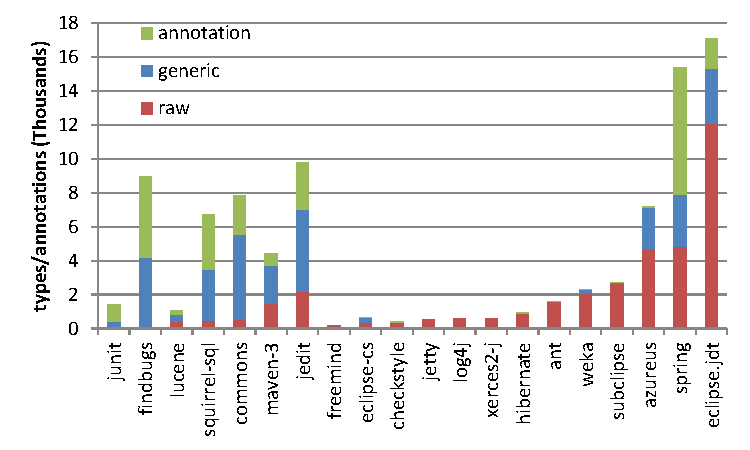
\includegraphics[width=\columnwidth]{oldProjectsUsage}
	\caption{Annotation, parameterized type, and raw 
			type counts in 20 established projects.}
	\label{fig:oldProjectsUseOfGenerics}
\end{figure}

\begin{figure}[htb]
	\centering
	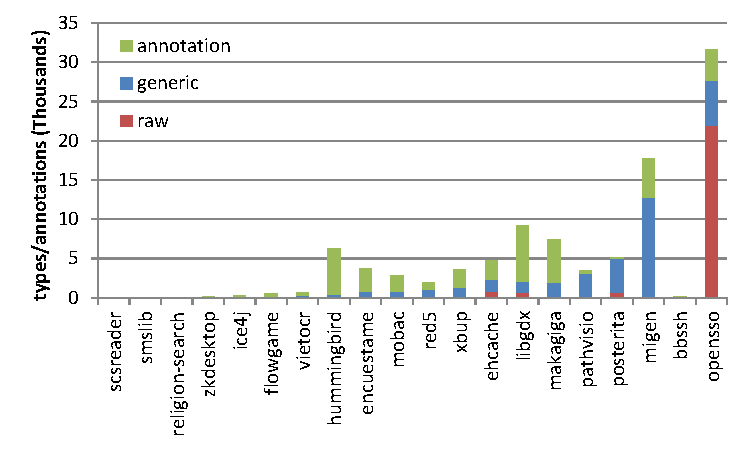
\includegraphics[width=\columnwidth]{newProjectsUsage}
	%\caption{8 projects out of 20 projects used generics prominently while the remaining 12 ignored generics in favor of raw types.}
	\caption{Annotation, parameterized type, and raw 
			type counts in 20 recent projects.}
	\label{fig:newProjectsUseOfGenerics}
\end{figure}


\subsection{Developers}

Did developers widely embrace generics? How did this compare with annotations?
We examined commits with creation or modification of parameterized types, 
generic type declarations, generic method declarations, or annotations.

\paragraph{Established projects.}In the established projects, 538 developers made 678,551 commits.
Of those developers, 71 made generic declarations (13\%), 128 specified annotations (24\%), and 141 used parameterized types (26\%).
%\todo{What does ``use generic declarations'' mean? created a generic decl? or created or used a decl?}
%For these developers, the average number of commits involving generic declarations was 27 commits and 554 commits associated with parameterized types.
Naturally, some developers commit more than others, which may give them more opportunity to use generics.  
Only 272 developers had more than 100 commits, averaging 2467 commits.  Within this group of 
more frequent committers, 66 used generic declarations (24\%), 99 used annotations (36\%), and 105 used parameterized types (38\%).

\paragraph{Recent projects.}In the recent projects, 232 developers made 197,744 commits.  
Of those developers, 47 used generic declarations (20\%), 138 used annotations (59\%), and 142 used parameterized types (61\%).
Of the 102 more frequent committers in the recent projects, with an average 1906 commits, 43 used generic declarations (42\%), 83 used annotations (81\%), and 87 used parameterized types (85\%).

The data suggests there were several forces shaping use of new features in Java by developers.  In both established and recent projects, a small minority of developers (perhaps with more authority or involvement) used generic declarations.  In most projects, a single member of a project (perhaps having an architect role) clearly
introduces a disproportionate amount of the generic declarations (see, for example, \autoref{fig:author-types}).
In established projects, developers demonstrated a modest use of generics and annotations.  Potentially, inexperience with the new features, or difficulty in migrating existing code to fit in with the new features hampered adoption.  In more recent projects, these factors may have been ameliorated, as a larger percentage of developers have started to use generics and annotations in their code.

In general, we observed that developers generally adopt usage of both features, although there were a handful of developers that only adopted use of either annotations or generics exclusively.

%reviewer2 didn't like forward references
% In later sections, we examine in more detail whether certain developers are choosing to ignore generics in favor of raw types (Section~\ref{sec:rawtypes}) and whether there is a 
% concerted effort to migrate those raw types to use generic types instead (Section~\ref{sec:migration}).
% max 25277, 

%maybe a table would fit in nicely here...

\subsection{Features Breakdown}

% Probably some more word smithing.
We characterize how different aspects of a feature were used
to identify any differences between established and recent projects
and between usage of aspects of those features.  
In both cases, these differences give insight into adoption factors,
such as the difficulty in learning aspects of a new feature 
and whether those differences persist over time. 
We focus mostly on generics, simply because there are many more aspects 
of generics to investigate in comparison with annotations.

\subsubsection{Common Parameterized Types}

We classified parameterized types as either user-defined
or from the standard Java Collections (\code{java.util}) based on name signatures.
We found that on the whole, use of Collections
types accounts for about 70\% of parameterized types across all of the codebases that we
examined.  %0.67814037
The most popular parameterized types across all projects
were \code{List}s, followed by \code{Map}s. 
\autoref{tbl:squirrel-sql-types-table}
illustrates this finding by showing use of 
the top 14 parameterized types in the \squirrelsql project.

\begin{table}[htb]
\centering

\begin{tabular}{lr}
\toprule
\textbf{Type} & \textbf{Parameterizations} \\
\midrule 
\texttt{List<String>} & 351\\
\texttt{ArrayList<String>} & 221\\
\texttt{HashMap<String,String>} & 157\\
\texttt{List<ITableInfo>} & 96\\
\texttt{Class<?>} & 91\\
\texttt{Collection<String[]>} & 77\\
\texttt{List<ArtifactStatus>} & 61\\
\texttt{Vector<String>} & 58\\
\texttt{List<ObjectTreeNode>} & 55\\
\texttt{List<TableColumnInfo>} & 55\\
\texttt{Iterator<String>} & 40\\
\texttt{List<Object[]>} & 33\\
\texttt{ArrayList<MappedClassInfo>} & 28\\
\bottomrule
\end{tabular}
\caption{Number of parameterizations of several generic types in \squirrelsql}
\label{tbl:squirrel-sql-types-table}
\end{table}

% CREATE view most_recent_revisions AS 
% (SELECT project,module,filename,MAX(datetime) as datetime FROM revisions GROUP BY project,module,filename);
% 
% CREATE view most_recent_revisions_without_deleted AS
% SELECT revisions.* FROM
% 		most_recent_revisions as m
% 	LEFT JOIN
% 		revisions
% 	ON
% 		m.project = revisions.project AND
% 		m.module = revisions.module AND
% 		m.filename = revisions.filename AND
% 		m.datetime = revisions.datetime
% 	WHERE
% 		revisions.state <> 'deleted';
% 
% SELECT [class_type] & "<" & [type_args] & ">" AS expr, parameterized_types.container_granularity, Sum(parameterized_types.Count) AS SumOfcount
% FROM most_recent_revisions_without_deleted INNER JOIN parameterized_types ON most_recent_revisions_without_deleted.FileID = parameterized_types.fileid
% GROUP BY [class_type] & "<" & [type_args] & ">", parameterized_types.container_granularity, parameterized_types.project
% HAVING (((parameterized_types.project)="squirrel-sql")) OR (((parameterized_types.container_granularity) Is Null))
% ORDER BY Sum(parameterized_types.Count) DESC;
% 		

In comparison, \autoref{tbl:squirrel-sql-annotations-table} illustrates how annotations were used in \squirrelsql,
showing a similar usage distribution to generics.
Annotations from the standard Java library, such as \textit{Override} and \textit{Before}, 
are the only annotations used by the majority of the 40 projects analyzed.
Otherwise, in addition to unit testing, annotations were used for a variety of domain- and project-specific cases.

\begin{table}[htb]
\centering

\begin{tabular}{lr}
\toprule
\textbf{Annotation} & \textbf{Use Count} \\
\midrule 

\texttt{Override} & 	1935 \\
\texttt{Test} & 	636 \\
\texttt{Before} & 	274 \\
\texttt{SuppressWarnings} & 		196 \\
\texttt{After} & 	158 \\
\texttt{Ignore} & 	16 \\
\texttt{GUITest} & 	4 \\
\texttt{Deprecated} & 	3 \\
\texttt{TestExecutionListeners} &		2\\
\texttt{RunWith} &		2\\
\texttt{ContextConfiguration} &		2\\

\bottomrule
\end{tabular}
\caption{Number of uses of annotations in \squirrelsql}
\label{tbl:squirrel-sql-annotations-table}
\end{table}

\subsubsection{Common Arguments}

We also investigated which type arguments were used most frequently.  
Again, there was a very clear dominant usage pattern.  
\code{Strings} were by far the most common arguments. 
\autoref{tbl:squirrel-sql-types-table} shows the
number of parameterized types of each kind of type argument in \squirrelsql for the most
commonly used types.  
In fact, it appears that \code{Lists} and 
\code{Maps} of \code{Strings}
account for approximately one quarter of parameterized types
in \squirrelsql.
% (2404 out of all 9072
% parameterized types in \squirrelsql).  
We observed similar patterns in other projects with generics, 
with \code{Collections} of \code{Strings} being the predominant parameterized type in
half of projects studied. %(18/36)
This trend tended to be stronger in the established projects, which predominantly 
used \code{String} parameters in 78\% of projects with generics, %(14/18)
compared to recent projects in only 22\%. %(4/18)
The second most popular parameter was \code{?} as an argument to the 
\code{Class} parameterized type, the most popular parameterized type in 14\% projects. %5/36
%why might that be?

\textbf{Overall, the most common usage of generics was to parameterize a collection of strings}.
%it might be nice to compare to annotations, but:
%		- the data we're getting from our framework is inconsistent; SupressWarnings, for instance,
%			should always take at least one argument, but it has none in the DB
%		- some annotations (e.g., override) take no arguments

%\subsubsection{Declarations}

%Figure~\ref{fig:generic_growth} displays the growth of generics over time.
%Each solid line represents the growth of generic type instantiations and each dashed
%line represents the growth of generic method and type declarations.
%Different colored lines represent different projects.

%Unsurprisingly, according to Figure~\ref{fig:generic_growth}, all projects use
%more instantiations than declarations, a trend that was consistent across most
%projects that we studied.
%The exceptions were freemind, jetty, log4j, and xerces2-j, none of which
%appeared to use generics at all. 

\subsubsection{Generic Types versus Methods}

We compared the number of user-defined generic types and methods across the established and recent projects.

\paragraph{Established projects.}In the established projects, 979 generic methods and 1684 generic types existed during the lifetime of the projects.
Out of the projects that used generics, 4 projects had fewer than 10 generic types, and 4 had more than 100 generic types.
This trend was not necessarily a function of size; for example, \findbugs made extensive use of generic types (116) in comparison to \jedit (39) even though \findbugs is roughly half the size of \jedit.
Figure~\ref{fig:decl-boxplot} shows box plots depicting the number of type and method declarations across all projects.
In all but 4 established projects there were more generic classes than generic methods, an almost 2-to-1 ratio. 
%A large selling point of generics was the ability to create generic operations over data. 
%Rather, we speculate that many generic types were used as placeholders and not as abstractions.
%That is, for many classes, the type parameter was being used 
%for a field inside the class and not necessarily for functionality of the class itself.

\begin{figure*}[t]
	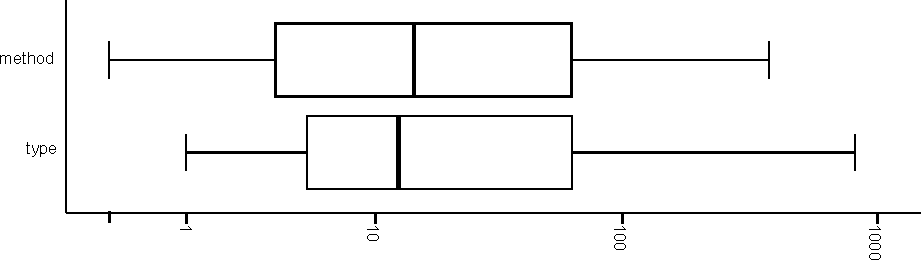
\includegraphics[width=\textwidth]{decl-boxplot.pdf}
	\caption{Box plots displaying the number of method and type declarations 
	in the projects under investigation.}
	\label{fig:decl-boxplot}
\end{figure*}

\paragraph{Recent projects.}In the recent projects, 666 generic methods and 1234 generic types existed during the lifetime of the projects.
Seven projects had fewer than 10 generic types, and 2 had more than 100 generic types.  Only 3 projects had more generic methods than generic types, again matching the near 2-to-1 ratio 
also seen in the established projects.  Overall, there were little differences between the established and recent projects.

%In total, 411 generic methods and 1127 generic types
%existed across all projects during the time of study.
%Out of the 15 projects that used generics, 
%6 had fewer than 10 generic types, 
%and 3 projects had more than 100.  
%This trend was not necessarily a function of size; 
%for example, \findbugs made extensive use of generic types (88) in 
%comparison to \jedit (33) even though \findbugs is vastly smaller.

A final observation we found was that introduction of generic types lagged behind the introduction of parameterized types, 
a tendency followed by most of the established projects that we studied.
Exceptions include an early adoptor of generics, \findbugs, which began using generic types and parameterized types
at about the same time, and \ant and \subclipse, 
which never used \emph{any} generic types. However, we did not observe this trend as strongly in recent projects.\todo{Bird, can confirm this?}
This lag suggests that \textbf{adoption may grow in stages as 
developers become more comfortable with the new feature}.
%We examine adoption lag in section~\ref{sec:adoptionlag}. 

\subsubsection{Unique parameterizations}\label{sec:uniqueparams}

For generics to be advantageous, each type declaration must 
be parameterized by multiple types, 
otherwise a simple non-generic solution would suffice.
But, for example, a generic type may be parameterized many times throughout the 
code but only have one unique parameter (\emph{e.g.,} \code{String}).  
In practice, how many unique parameterizations are made of type declarations?
Is the number small or are generics preventing thousands of clones from being created? 
From our data, we counted user-defined type declarations and their parameterizations.
Figure~\ref{fig:unique-boxplot} shows box plots depicting the 
number of parameterizations of each user-defined type.

\begin{figure*}[t]
	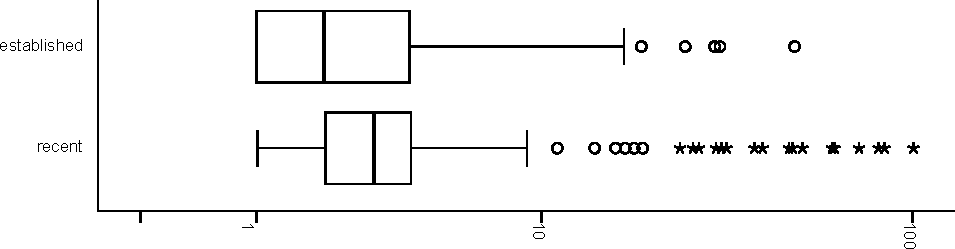
\includegraphics[width=\textwidth]{unique-boxplot.pdf}
	\caption{Box plots displaying the number of parameterizations
	of each user-defined type in the established and recent projects.}
	\label{fig:unique-boxplot}
\end{figure*}


\paragraph{Established projects.}In our established projects, 330 user-defined generic type declarations were instantiated in total 1123 times.  
Of those, 38\% had a single parameterization.
The remaining 62\% ranged from 2 to 49 parameterizations (mean=4.8). 
The distribution was very positively skewed such that 80\% of generic classes had fewer than 5 parameterizations.

\paragraph{Recent projects.}In our recent projects, 332 user-defined generic type declarations were instantiated in total 2027 times. 
Of those, 23\% had a single parameterization.  The remaining 77\% ranged from 2 to 100 parameterizations (mean=7.5).
Still, 76\% of generic classes had fewer than 5 parameterizations.  

Overall, the lower portion of the distribution for both the established and 
recent projects were similar, differing on the tail-end in magnitude.
This suggests that the \textbf{cost savings envisioned by the language designers
may not have been fully realized in practice}. 
%We investigate further in Section~\ref{sec:codedup}.

\subsubsection{Advanced Parameterizations}

We examined several advanced uses of parameterization,
including \textbf{wildcard types}, such as \code{List<?>}, 
where the type argument matches any type;
bounded types, such as \code{List<? extends Integer>}, 
where the argument matches a certain set of types;
nesting, such as \code{List\textless List\textless String> >};
and multiple type arguments such as \code{Map<String,Double>}.

\paragraph{Established projects.}As a percentage of all parameterized types for the established projects, 
each advanced use made up the following percentages:
nesting (\textless 1\%),
bounded types (4\%), 
wildcards (11\%), and                                                                                                                         
multiple type arguments (22\%).
\paragraph{Recent projects.}The break down was similar for the recent projects, as a percentage of all parameterized types  
each advanced use made up the following percentages:
nesting (\textless 1\%),
bounded types (2\%), 
wildcards (15\%), and
multiple type arguments (14\%).

The consistent levels of usage between established and recent projects suggests that \textbf{there was an inherent difficulty or limited applicability in the more advanced features of generics, 
limiting their adoption}.

\section{Investigating Claims}\label{sec:claims}

In this section, we examine \autoref{hypo:cast_reduction} and 
\autoref{hypo:codedup_reduction}.
Here we do not specifically compare results for 
established projects against those for recent projects,
as we did not find any substantial
differences between the two project sets.

\subsection{Generics reduce casts}\label{sec:castsvsgenerics}

%Is there a mathematical test that we can do here? Some sort of correlation?
% it would seem that if we have just the change in the number of casts per
% transaction, we could correlate that with the number of generics

\begin{figure*}

	\centering
	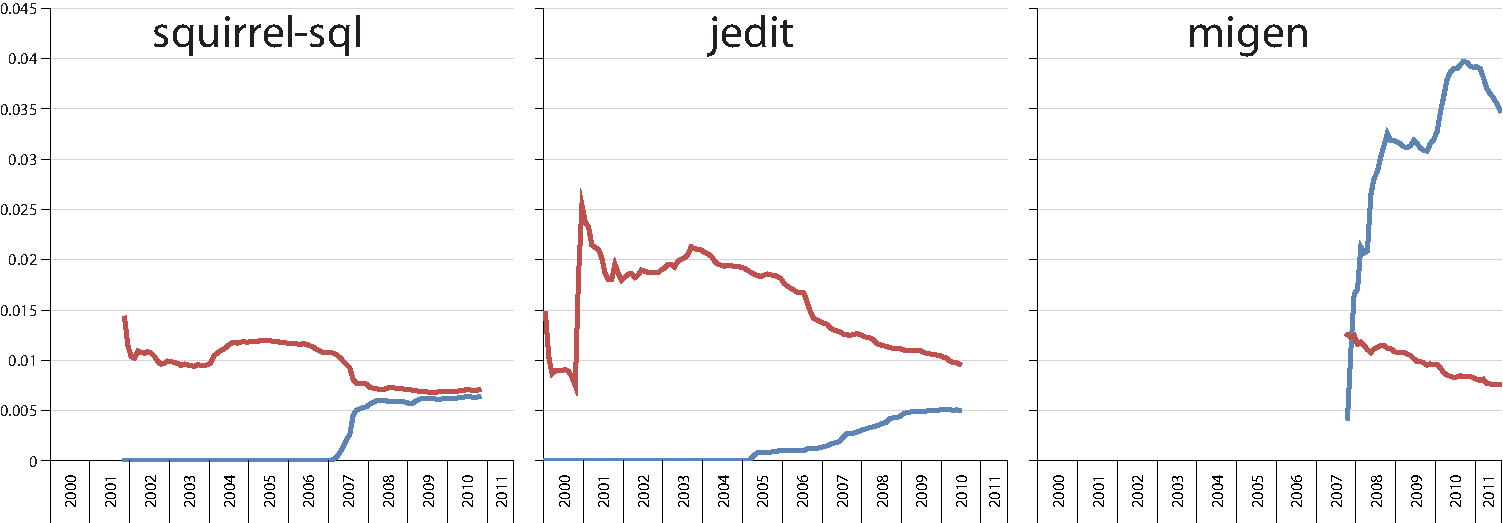
\includegraphics[width=\textwidth]{casts_vs_generics}
	
	\caption{Casts (red, top line) and parameterized 
	type (blue, bottom line) density.  Parameterized type density is scaled
    by a factor of ten to aid visual comparison.}\label{fig:casts_vs_generics}
	\todo{use different colors}
\end{figure*}


An argument for introducing generics is that they
reduce the number of runtime exceptions because they reduce
the need to cast (\autoref{hypo:cast_reduction}).
Thus, it is reasonable to expect that the addition of generics
will reduce casts.

To test \autoref{hypo:cast_reduction}, we examined 
our data to determine if an increase in generics leads to a
decrease in casts.
However, comparing just the raw number of generics against the 
raw number of casts could be misleading, because an increase in 
generics may not actually cause a decrease in casts whenever new 
code containing parameterized types is added.
To control for this, we calculated the density of program elements 
(parameterized types or casts) by dividing the number of 
program elements by Halstead's program length~\cite{halstead}.
Halstead's program length is the sum of the total
number of operators (such as method calls)
and the total number of operands (such as a variable).
We used Halstead's program length here 
because it measures program size, but also  
disregards code formatting, whitespace and comments, making
it preferrable to a simple lines-of-code metric.
Thus, Halstead's program length allows us to more fairly compare 
projects that use different conventions for formatting,
whitespace, and comments.
This is important because, for example, \azureus has about half has many
comments per line of code as \weka, according to \url{ohloh.net}.

Figure~\ref{fig:casts_vs_generics} plots the cast and parameterized type density 
for three projects.
%see casts_vs_generics
The x-axis represents time and the y-axis is the density of program elements.
The number on the y-axis represents the number of program elements 
per unit program length.  Red (top) lines represent the density of casts over time.
Blue (bottom) lines represent the density of parameterized types over time.
Because the density of parameterized types is small relative to that of casts, 
to improve the readability of the figure, the blue line is scaled by 10.
Similar time series graphs are shown in the Appendix for all projects.

Overall, the graphs do suggest a relationship between the use of casts
and the use of parameterized types.
In \squirrelsql, an increase in generics in 2007 corresponds to a 
decrease in casts.
The same is true about \jedit from 2005 onward and over the lifetime of \migen. 
Ten other projects also distinctively showed this trend
(\ice,
\eclipsecs,
\flowgame,
\findbugs,
\junit,
\lucene,
\maven,
\mobac,
\spring, and
\pathvisio).
Interestingly, a few projects showed the opposite trend
(\religion, \libgdx, \hummingbird, \commons), where increases in generics
tended to correspond to increases in casts.
We speculate that this opposite trend may be due to 
changes that require use of generic types and 
APIs that require casting.
For instance, using Java's reflection API, 
the object returned from \texttt{Class.forName(\ldots)} 
will likely need to be cast.
% \begin{itemize}
% \item
% The number of casts fluctuates significantly in the initial
% phase of all three projects (a trait shared by most of the 20 projects that 
% we investigated), even before the introduction of generics.
% It would appear that some software development practice has a larger effect 
% on casts than parameterized types.
% %it could be that the fluctionation is largely due to the program being initially small, no? 
% \item
% After the initial turmoil, all three projects show a gradual decline in the number
% of casts (a trait shared by about half of the projects that we investigated), 
% \emph{even before developers start to introduce generics}.
% This suggests that some other software development practice reduces the 
% number of casts in a project over time.
% \end{itemize}
% 
% However, the figures do suggest that the introduction of generics may, in some
% circumstances, reduce the number of casts.
% Specifically, notice that \eclipsecs and \squirrelsql both exhibit sharp increases
% in the number of generics.
% \eclipsecs, and to a lesser extent \squirrelsql, simultaneously decrease the number of casts
% in the program.
% This suggests that some projects will see a decrease in the number of casts when generics
% are introduced.
% However, this effect seems to be limited; a total of 6 out of 15 projects that used generics 
% ever exhibit this sharp inverse relationship.

In addition to a visual inspection, we used Spearman's rank correlation to
examine the relationship between generics density and cast density over time. 
We also employed Benjamini-Hochberg p-value correction to mitigate false discovery~\cite{benjamini1995cfd}. 
Only \religion did not show a statistically significant correlation ($p > .05$).
Of the remaining 35 projects that used generics, we found that:
6 projects showed a strong inverse correlation (above $-0.84$);
9 showed a moderate inverse correlation (between $-0.4$ and $-0.8$); and
8 showed a weak inverse correlation (between $0$ and $-0.4$).
However,
10 projects showed a weak positive correlation (between $0$ and $-0.4$)
while, surprisingly, 
\makagiga ($0.69$) and \encuestame ($0.65$) showed strong positive correlations,
indicating that increased generics use coincided with more casts.
Again, this positive correlation may be due to changes
that require use of generic types and APIs that require casting.

On the whole, the data that we collected 
\textbf{supports}~\autoref{hypo:cast_reduction}.

One limitation to this analysis is that we considered 
trends across all contributors.
While this illustrates a more project-wide trend, it may be that if we considered only the
trends of generics and casts for developers who embraced generics, there would be a stronger
relationship.

Another limitation is that our density function used in the 
cast analysis sometimes may not accurately measure the effect of parameterized types on
casts.
For example, if a program contains generics, and then a large class is deleted that contains many casts and
no generics, the density of generics in the program goes up while the density of casts goes down.
Our analysis would mis-interpret this change as the addition of generics causing the removal of casts.
Further study with more sophisticated metrics are needed to mitigate this threat.

%Limitations: do not discount generic casts (but probably not too many) (?)

\subsection{Generics prevent code duplication}\label{sec:codedup}

Another claim regarding generics is that a generic type \code{Pair<S,T>} would
prevent the need for countless clones of classes such as \code{StringIntPair}
and \code{StringDoublePair} if a developer wanted to create a type-safe
container.  But in practice, how many clones would actually be needed?  How
many duplicated lines of code and bugs would be introduced from having to
maintain these clones?

To test \autoref{hypo:codedup_reduction}, we measured the number of unique
parameterizations for all parameterized types to determine the number of
clones.  Further, we take our previous measures of unique parameterizations of
just user-defined generics (shown in Section~\ref{sec:uniqueparams}), and use the
lines of code and number of revisions in the source repository to estimate the
impact of code duplication.  
Total lines of duplicated code are calculated by
taking the number of unique parameters (P), lines of code (LOC)
and applying this formula: $D = LOC *  (P - 1)$.  This estimates the
amount of additional code needed to provide implementations of non-generic code for each
type parameter, $P$.
Next, we take the total
duplicated lines (D), the number of revisions (R), and an error constant (K) to
estimate the potential faults in the code in this manner: $E = D * R * K$.  This is a
rough estimate that assumes a relatively uniform bug rate across lines of code.

From our 40 projects, we found a large number of clones would need to be created for a small number of types.
We observed parameterization of 1152 types, but actually found about 
46\% of these types (532) only had exactly one type argument ever used
throughout the project's history, 
suggesting that needless or premature generification of objects occurs fairly frequently.
From the top ten generic classes having the most parameterizations (all were Java collection classes), we found a total of 8686 different parameterizations.
To accommodate all the parameterizations of these ten classes, 8676 clones would need to be created, or about 868 clones per class.  
But the number of parameterizations dropped drastically for the remaining 1142 classes; 5275
 clones would need to be created, or about 4.6 clones per class.  
Interestingly, we only found 13 parameterizations of \code{Pair} types across all projects.
We speculate that a generic version of \code{Pair} is less useful than we
initially expected.
%SELECT c,count(*) FROM
% (SELECT REPLACE(class_type,"java.util.","") as c,type_args from parameterized_types
% GROUP BY REPLACE(class_type,"java.util.",""),type_args) as _
% GROUP BY c
% ORDER BY count(*) DESC;

Next, we analyzed the user-defined generic class from 
each project that had the most parameterizations,
for the purpose of estimating the impact of code duplication.
In total, we analyzed 12 user-defined generic classes from
the established projects and 12 from the recent projects.
The generic classes had a total of 347 parameterizations.  
The mean code size of the classes was 176 lines of code and the classes 
were changed a total of 244 times (mean 10).
%The 109K number below includes negative numbers from classes with no uses
We estimate, as a result from these 24 generic classes alone, an estimated 109,816 lines of duplicated code were prevented.  
With our error estimation, 195 errors would have been prevented based on our metric and an error constant of 7.4/100000 
(1/100 errors per commit, and 7.4/1000 errors per LOC~\cite{Humphrey:1995}).
However, the number of errors prevented varied significantly between 
generic classes; of the 24 total generic classes, 
we estimate that 16 of them prevented no bugs at all.

Overall, this \textbf{supports \autoref{hypo:codedup_reduction}}; 
however, the impact may not have been 
as extensive as expected.
The benefit of preventing code duplication is largely confined 
to a few highly used classes.

Using a Wilcoxon signed-ranks test, we observed that
there were no significant differences between the
set of 20 established projects and the set of 20 recent projects.
More specifically, there were no significant differences
in terms of either group's 12 user-defined generic types 
in any of the following metrics:
lines of code, duplication prevented, or errors prevented.
This suggests that projects that ``grew up with generics''
did not benefit from generics' duplication prevention
any more than established projects.

There are limitations to our results.  
We may over-estimate the code duplication if inheritance could have shared non-generic methods.
We may under-estimate the number of unique parameterizations, as some generic types are intended for client use and were not used in the code we analyzed, for example the library \commons; there were 674 generic classes that were never parameterized.
Further, we excluded 119 generic types from analysis that had only one unique parameter which themselves were other generic parameters.  
This might be common, for example, with a \code{GenericHashKey} that might be used by other generic types.
Finally, we did not exclude generics that were introduced for testing purposes,
such as in \jdt, where some generics are used to test Eclipse's Java language tools.
As a consequence, projects that used generics for testing may not be representative
of the average Java project.

\section{Factors for Adoption}\label{sec:adoption}

Risk, legacy code, backward compatibility, developer politics, feature complexity, and learning;
these are several factors that may influence adoption.  By comparing differences in adoption by established and recent projects of generics and annotations 
we attempt to tease apart some of these factors.

\subsection{Do developers change old code to use new features?}\label{sec:rawtypes}
\label{section:old-code}

\begin{figure*}[t]
	\subfloat[\squirrelsql]{\includegraphics[width=0.33\columnwidth,page=13]{types-plots}}
	\subfloat[\jedit]{\includegraphics[width=0.33\columnwidth,page=5]{types-plots}}
	\subfloat[\migen]{\includegraphics[width=0.33\columnwidth,page=29]{types-plots}}

	\caption{ 
	  Migration efforts in switching old style collections was mostly limited in projects: old code remains.
		Solid lines indicate use of raw types (types such as \code{List} that 
		provide an opportunity for generification) and dashed lines, generic types.}
	\label{fig:raw-migration}
	\vspace{-12pt}
\end{figure*}

Since generics supposedly offer an elegant solution to a common problem, we
investigated how pre-existing code is affected by projects' adoption of
generics in an effort to answer \autoref{hypo:migration}.  
Conversely, for this research question, we did not examine annotations, as there was 
no corresponding old feature to ``upgrade''.
Is old code modified to use generics when a project decides to
begin using generics?  There are competing forces at play when considering whether to
modify existing code to use generics.  Assuming that new code uses generics
extensively, modifying existing code to use generics can make such code
stylistically consistent with new code.  In addition, this avoids a mismatch in
type signatures that define the interfaces between new and old code.  In
contrast, the argument against modifying old code to use generics is that it
requires additional effort on code that already ``works'' and it is unlikely
that such changes will be completely bug-free.  
% CP: Let's, save this for FSE when we have hetergenous results.
%Further, some projects may use
%container classes that appear to be candidates for generification in a way that
%is actually not amenable.  For example, using lists as tuples of heterogenous
%types.

To address this question as presented in \autoref{hypo:migration}, 
we examined if and how old code is modified after
generics adoption.  \autoref{fig:raw-migration} depicts a gross comparison by
showing the growth in raw types (solid red) and generic types (dashed blue)
over time for the three projects of interest (see Appendix for graphs of all projects).
Note that raw types are types used
in the system for which a corresponding generic type exists, such as List.
A drop in raw types that is
coincident with an increase in parameterized types (e.g. in mid 2007 in \squirrelsql,
which we manually verified by inspection as a large generification effort)
indicate evidence of possible generification.  Changes in types may not
themselves be evidence of actual generification, however.  We therefore
determined generifications in a more principled way.  Specifically, we
identified raw types in the code as candidates for parameterization.
We then examined what proportion of these candidates actually were removed and
replaced by their generic counterparts by using the approach described in
Section~\ref{section:find-migrations}.

%jedit - 517 generifications, final 2830 raw types, 4477 ptypes, 4360 cum raw types
%squirrel-sql - 574 generifications, final 727 raw types, 2947 ptypes, 1411 cum raw types
%eclipse-cs - 30 generifications, final 466 raw types, 299 ptypes, 497 cum raw types
%commons - 867 generifications, 3102 cum raw types
%lucene - 794 generifications, 2380 cum raw types

\paragraph{Established Projects.}
Consider \squirrelsql\textemdash~a total of 1411 raw types were introduced into the codebase
over the life of the project (note that some were removed before others were
added, so the maximum shown in \autoref{fig:raw-migration} is 1240).  Of these,
574 (40.7\%) were converted to use generics over a five month period starting
when they were adopted in early 2007 (we identified these using the approach
described in Section~\ref{section:find-migrations}). In contrast, \jedit had 517 of a total of 
4360 introduced raw types converted to use generics (11.9\%). 
Of the other projects studied, only \commons
(28\%) and \lucene (33.4\%) had more than 10\% of their existing raw types
generified.  In aggregate, only 3 of the 15 projects that use generics
converted more than 12\% of their raw types and none of them converted more than
half of their raw types use.
We therefore conclude that although we do see a few large-scale migration efforts,
\textbf{most projects do not show a large scale conversion of raw to parameterized types}.

\paragraph{Recent Projects.} For recent projects, we see
even fewer and smaller migration efforts. In the \red project, 134 of the 416
total raw types that were added were eventually converted to parameterized
types (yielding a final total of 1082 parameterized types).  No other recent
projects had more than 100 raw types converted to parameterized types, and seven
projects had no migrations at all.

The reasons behind the lack of migration in the established and recent projects may actually be
different.  For projects that had a substantial code base when generics were
added to the language, raw types were already heavily used and thus developers
decided not to modify that code, taking an ``if it's not broken, then don't fix
it'' mentality.  In contrast, most projects that started after 2005 used
generics from the start and did not use raw types extensively to begin with
(notables exceptions were \ehcache and \bbssh).  In these projects, we did not
see migrations because there was not a large set of raw types that \emph{could}
be converted to use generics.

\subsection{Who buys-in?}\label{sec:migration}

\begin{figure*}[ht]
	\subfloat[\squirrelsql]{\includegraphics[width=0.33\columnwidth,page=13]{author-plots}}
	\subfloat[\jedit]{\includegraphics[width=0.33\columnwidth,page=5]{author-plots}}
	\subfloat[\migen]{\includegraphics[width=0.33\columnwidth,page=29]{author-plots}}
	
	\caption{Contributors' introduction and removal of type uses over time for the five most active contributors in each project. 
		Solid lines indicate use of raw types (types such as \code{List} that 
		provide an opportunity for generification) and dashed lines, parameterized types.  Each color represents a different contributor.}
	\label{fig:author-types}
	\vspace{-12pt}
\end{figure*}


\autoref{hypo:community_acceptance} relates to \emph{who} uses a new feature in the
projects that adopt them.  We expect that since most large projects depend on
the principle of community consensus, the decision to use a new feature would
be made as a group and would not be dominated by one developer.  We separately analyzed 
developer's use of generics and annotations.  We also looked for any differences between 
established and recent projects, where the \emph{newness} of a feature may affect the dynamics of how community consensus occurs.

To answer \autoref{hypo:community_acceptance}, we first examined the introduction 
and removal of a feature by developers over time.
We performed a Fisher's exact test~\cite{dowdy2004sr} of
introduction of raw and parameterized types comparing the top contributor 
with each of the other contributors in turn (using Benjamini-Hochberg
p-value correction to mitigate false discovery~\cite{benjamini1995cfd}) to determine
if any one contributor uses a feature on average much more than the others.  This test
examines the \emph{ratio} of raw types to parameterized types rather than the total volume,
so that the difference of overall activity is controlled for.

To illustrate these results, we make use of several graphs detailing different author's usage of a feature in a project.
\autoref{fig:author-types} shows the introduction (and removal)
of parameterized types by contributor for the five most active contributors to each
project.  A solid line represents the number of raw types, which are candidates for
generification, and a dashed line, parameterized types. Pairs of lines that are the same color
denote the same contributor.   A downward sloping solid line 
indicates that a contributor removed raw types.  
For instance, \ref{fig:author-types}-a shows that in \squirrelsql, one contributor began introducing 
parameterized types in early 2007 while concurrently removing raw types.  
The Appendix contains similar graphs of all projects.

\paragraph{Contributors' Use of Generics.} The most common pattern that we observed across projects was
one contributor introducing the majority of generics.  
This pattern is illustrated in \squirrelsql (\ref{fig:author-types}-a) and similar phenomena were observed in \eclipsecs, \jdt,
\hibernate, \azureus, \lucene, \weka, and \commons.  
In established projects, one contributor dominates all others in their use of parameterized types 
to a statistically significant degree ($\alpha=.05$).

In recent projects, we hypothesized that there may be different phenomena at work since there
was no pre-existing non-generic code base that would make the decision to use
generics a debated topic.  Therefore, we expected broad community usage of
generics.  However, even in these newer projects, there was still a clear
champion that accounted for most generics use in all but two projects (the
contrary projects were \pathvisio and \scsreader).

There were some outliers.  \jedit (\ref{fig:author-types}-b) represents a less common pattern in that all
of the active contributors began using generics at the same time (towards the
end of 2006).  This is more representative of \spring, \junit, and \maven.
Although our graph of \jedit shows that most contributors began
using parameterized types, a Fisher's exact test showed that one contributor
%(Shlomy Reinstein, 
(shown in yellow) still used parameterized types more often than raw types
compared to all other contributors to a statistically significant degree.
Lastly, \findbugs (not shown) is an outlier as the two main contributors 
%,Bill Pugh and David Hovemeyer,
began using generics from the very beginning of
recorded repository history and parameterized types were used almost exclusively where
possible; we found almost no use of raw types in \findbugs at all.

\paragraph{Contributors Use of Annotations.}
As a contrast to our generic buy-in results, we also
examined individual contributors' adoption of annotations.  
Consistent with our results of analysis
individuals' adoption of generics, we found that the majority of the projects that used annotations had
a clear ``champion'' that used them more than the rest of the contributors to a statistically significant degree.
\autoref{fig:author-annotations} shows the adoption graphs for the most active contributors in three projects.
The graphs for the \jdt and \libgdx projects are representative of the vast majority of projects, as there is an obvious
contributor that accounts for most annotations.  The graph for \migen is uncharacteristic, as there were a number of 
contributors that all actively added annotations to the codebase at roughly the same rate and time interval.
Annotation graphs for all projects are shown in the Appendix.

\begin{figure*}[ht]
	\subfloat[\jdt]{\includegraphics[width=0.33\textwidth,page=10]{author-annotation-plots.pdf}}
	\subfloat[\libgdx]{\includegraphics[width=0.33\textwidth,page=39]{author-annotation-plots.pdf}}
	\subfloat[\migen]{\includegraphics[width=0.33\textwidth,page=29]{author-annotation-plots.pdf}}
	\caption{Contributors' introduction and removal of annotations over time for the most active contributors in each project. 
		Each color represents a different contributor.}
	\label{fig:author-annotations}
	\vspace{-12pt}
\end{figure*}

The reader may notice that each of these graphs shows occurrences of steep
increases over short time periods (e.g., the user sergut in \migen in the early
part of 2011).  Interestingly, we also observed abrupt introductions of hundreds
and sometimes even thousands of annotations in very short time periods.  For
instance, one contributor in the \lucene project added 2,182 annotations
(across multiple files) in just one commit and one contributor added 16,019 to \hummingbird
in just two days!  
We speculate that this level of activity may be indicative of use of an automatic technique for adding annotations.  
While not quite as extreme, we observed ``bursts'' of
annotation introduction (usually on the order of hundreds in a short time period)
in all projects that actually used annotations (36 out
of 40) except for \makagiga, which showed a fairly constant monotonic increase, and \weka and \ant, which did not 
use annotations extensively.

Overall, the data and our analysis indicates that \textbf{features are usually
introduced by one or two contributors who ``champion'' their use and broad adoption
by the project community is uncommon}.

In further work, we plan to investigate and contact
these early adopters to identify \emph{why} and \emph{how} they began
introducing new features as well as the obstacles (both technological and social)
that they encountered.

\subsection{What factors affect adoption?}\label{sec:adoptionlag}

% Introduction.
Is backward compability the dominating concern, or do other factors such as risk, learning, or tool support play a role as well?
In legacy codebases, are less risky features adopted earlier than more risky features?  Do these trends disappear in more recent projects?

%We next turn to the question of how long it has taken software projects
%to adopt generics or annotation use and if there is a relationship with the legacy code, JVM compatibility, tool support (including IDEs
%such as Eclipse and NetBeans) of generics and annotations.  In order to relate time to key events
%that may affect adoption, we chose dates of generics feature introduction in Java and IDE support for generics.

To evaluate \autoref{hypo:ides}, we focused on the factors of compatibility and IDE support.
We separately analyzed established and recent projects where applicable to identify consistent trends.

%\autoref{table:ides}
%shows shows the IDEs that we were able to identify for each project.
%\begin{table}
%\centering
%\begin{tabular}{ll}
%\toprule
%\textbf{Project} & \textbf{IDE} \\
%\midrule
%\ant & Unknown \\
%\azureus & Eclipse \\
%\checkstyle & Eclipse, V IDE \\
%\commons & Unknown \\
%\eclipsecs & Eclipse \\
%\findbugs & Eclipse \\
%\freemind & Unknown \\
%\hibernate & Unknown \\
%\jedit & jEdit \\
%\jetty & Eclipse \\
%\junit & Eclipse \\
%\logfourj & Unknown \\
%\lucene & Unknown \\
%\maven & Unknown \\
%\jdt & Eclipse \\
%\spring & Eclipse \\
%\squirrelsql & Eclipse, IntelliJ IDEA \\
%\subclipse & Eclipse \\
%\weka & Eclipse \\
%\xerces & Eclipse \\
%\bottomrule
%\end{tabular}
%\caption{IDEs used by each project}
%\label{table:ides}
%\end{table}


\subsubsection{Compatibility or Other Factors}

To evaluate the factor of compatibility, 
we examined the difference between adoption dates of annotations and adoption dates of generics. Our reasoning is that if concerns of compatibility was the primary factor holding back adoption,
then we should observe near simultaneous adoption of both features once the concerns had been removed.  Alternatively, if we observe large differences in adoption dates between the features, 
then some other factors may had held back adoption of a particular feature.

%Feature complexity, legacy code (established).
\paragraph{Non-simultaneous adoption in most Established Projects.} We examined the dates of the first annotation and generic used in the established projects.
Although we did find a few projects that introduced annotations and generics simulanteously,
the majority of projects staggered adoption, often by years.
Specifically, we found 4 projects adopted generics before annotations, ranging from months to years  
while 7 projects adopted annotations before generics, ranging from several days to years (for \subclipse annotations appeared 5 years before the first generic). Interestingly, \logfourj introduced annotations in 2007, but never introduced generics. There were 5 projects that first used annotations and generics on the same day.
Overall, established projects staggered adoption between features by an average of 296 days.
Figure~\ref{fig:time-boxplot} shows box plots depicting the number of days between
adoption of generics and annotations.

\begin{figure*}[t]
	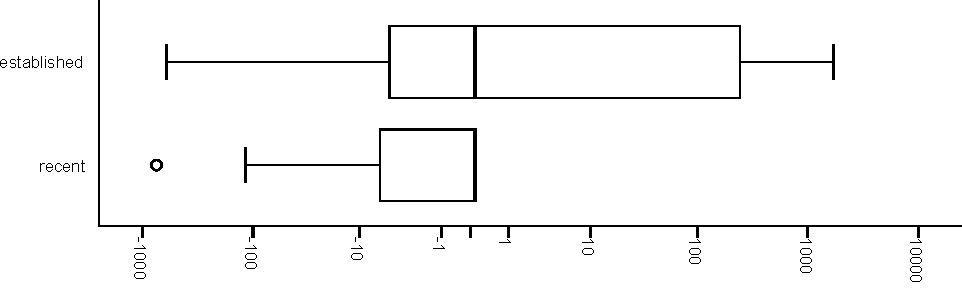
\includegraphics[width=\textwidth]{time-boxplot.pdf}
	\caption{Box plots displaying the number of days between when generics were
	introduced and when annotations were introduced in established and recent projects.
	Negative values indicate that annotations were introduced before generics.}
	\label{fig:time-boxplot}
\end{figure*}

	\paragraph{Near-simultaneous adoption in Recent Projects.} Interestingly, the trend seen in established projects does not hold for recent projects.
	Instead, the recent projects were much quicker to use both features in a near-simultaneous fashion. 
	We found 6 projects used generics before annotations, ranging from days to months, while 14 projects use annotations and generics on the same day.
There was a near-simultaneous adoption of annotations and generics (an average 53 days lag), suggesting that projects used the available features in a major language upgrade together.
This delay of 53 days is significantly shorter than the 296 days experienced by established projects (p \textless .02 by an unpaired 2 tailed t-test).

\smallskip
If compatibility was the sole important factor, we might have expected more simultaneous adoption.
Still, we do believe compatibility plays a role.  For example, we did see examples of people holding back code (\emph{e.g.}, \texttt{List/*<String>*/}) and a few projects adding in both features 
on the same day.  Further, there is evidence of delay between the release of Java 5 and adoption of either annotations or generics. 
We found an average adoption lag of 500 days after the official release by the established projects.
However, other factors delay adoption even further (an average 296 days).

Overall, from the data that we collected to answer if compatibility is the sole factor in~\autoref{hypo:ides}, 
the results indicate that \textbf{compatibility is an important, but not sole factor in adoption and other factors such as legacy code may contribute to even further delays}.

\subsubsection{IDE Support}

To evaluate IDE support, we first had to determine which projects used
which IDEs and were active prior to IDE support (the 20 established projects).  
We found evidence that IDEs were used for development for most of the projects that we studied.  This
evidence existed in the form of files created by IDEs (\code{.project} files in
the case of Eclipse) or discussions on mailing lists.  Eclipse was the most
predominant IDE that we found evidence for, used by developers in
\azureus, \checkstyle, \eclipsecs, \findbugs, \jetty, \junit, \jdt,
\spring, \squirrelsql, \subclipse, \weka, and \xerces.

Although Java 5 with generics was released in September of 2004, Eclipse
did not support generics until the public release of version 3.1 in late June,
2005.  NetBeans supported generics at the same time that they were introduced, making a study of the
effects of support for this IDE difficult if not impossible.
We therefore examined each of the eight established projects that use Eclipse as an IDE to
determine if they adopted generics prior to the 3.1 release.  Of these
projects, \checkstyle, \junit, \jdt and \findbugs started using generics prior
to generics support in Eclipse.  The other four projects waited until
after generics support appeared in Eclipse and did not switch until sometime in 2006 or later (\subclipse
did not begin using generics until 2010).  We examined the developer mailing lists at the time
that generics support was added to Eclipse and also at the time that they began using generics
and found no discussion of generics support in Eclipse as a factor in decision-making.
Although these eight projects technically adopted generics after Eclipse support for them,
the fact that adoption did not occur for at least six months after such support along
with an absence of evidence on the developer mailing lists, leads us to believe that IDE support
may not be critical.

The following quote from Jason
King in a discussion of generics support in Eclipse
provides one way to reconcile the perceived importance of tool support with 
our findings.\footnote{\scriptsize{\url{http://www.theserverside.com/news/thread.tss?thread_id=37183}}}

\begin{quote}
Our team adopted Java 5.0 back in November 2004 and incrementally adopted the
[Eclipse] 3.1 milestone builds as they came out throughout the first 6 months of this
year. We found the product to be remarkably stable from an early stage, with
few serious bugs.

As the entire team was learning the Java 5 features, we started manually coding
in generics (and enums, varargs, annotations etc). A few times we complained
that autocompletion and refactoring would help, but the absence didn't stop us.
When a new [Eclipse] milestone came out our pairing sessions were really fun as we
discovered new features appearing in the IDE.
\end{quote}

Although tool support does not appear to be critical, we also looked at
time of adoption to identify other possible factors affecting
uptake time.  
However, we found no trend related to when generics were adopted.
For instance, \jedit started using them
in 2004, \squirrelsql in 2006, \eclipsecs in 2008, and \subclipse in 2010.
\findbugs is again an anomaly as it used generics \emph{before generics were officially
released}!  The only statement we \emph{can} confidently make is that there was
\emph{not} strong adoption of generics immediately following their introduction
into Java.

We also saw wide variation in the \emph{rate}
of generics adoption within the codebases.  \autoref{fig:raw-migration} shows that
\squirrelsql and \jedit introduced generics into the code at a rapid
rate once the decision to use them was made.  
A number of projects, 
\lucene, \hibernate, \azureus, \checkstyle, and \junit show a lull in generics use
for months or even years following first generics use.  
\migen, a recent project, is shown in \autoref{fig:raw-migration} 
to illustrate a recent project where no migration took place.
%TODO was there really no migration in migen, or negligible?

Overall, the data that we collected to answer the factor of IDE support in~\autoref{hypo:ides}, 
the results indicate that \textbf{lack of IDE support for generics
did not have an impact on its adoption}.  This
finding raises more questions than it answers.  Deciding to use a new language
feature is non-trivial and can have large consequences.  If many projects
adopted generics, but did so at vastly different times and rates, what factors
affect the decision of when to begin using them?  In the future, we plan to
contact project developers, especially those that first began using generics,
to identify these factors.  Finally, although we did not investigate tool support for annotations, we did observe several instances were annotations appeared to be introduced via tool support.

\section{Limitations}\label{sec:limitations}

There are several threats to validity in this study.

\paragraph{External Validity}
The projects we have sampled are all open-source projects, and they may not be representative of all software development projects.
For example, certain industries, such as the defense industry, 
have stricter standards and slower timelines in supporting new versions of software, such as language runtimes, 
which may amplify or alter the conclusions of the study.

Even within open-source projects, the number of projects and the type of categories we have selected from 
may not be sufficient to draw conclusions for all open-source projects.  Although, the data we have examined 
has highlighted several significant results, future research should confirm these findings at a larger scale within the open-source community.

\paragraph{General Validity}
The conclusions of this study are particular to adoption of language features in Java and may not hold for other languages.
For example, a parallel adoption story of generics exists in C\#\textemdash generics were also introduced in a new version of the language; 
however, subtle differences in the design and deployment of C\# generics may have resulted in a different adoption story.

Further, the conclusions about the language features we have examined\textemdash Java generics and annotations\textemdash 
may not extend to other newly introduced language features such as Java closures.  
Future research needs to draw parallels between differences in adoption of language features 
and channel differences as insight into future design of language features.

\paragraph{Construct Validity}
Several conclusions in our study rely on complex analysis techniques.
Limitations in those analysis techniques may have caused some results to be underestimated.
For example, the migration analysis relies on the assumption that a raw type is migrated to a generic type if the fully qualified name of the method remains the same across revisions.
This assumption may fail to count migrations that occurred during structural changes such as a file or signature rename.
Note, that this assumption is not used for the other analyses, which tracks features at a project-wide level per revision.

In other cases, an analysis may only offer one perspective on the data when multiple 
perspectives might be needed.  For example, one limitation of the cast analysis is that it is coarse-grained, 
examining the general relationship of casts and generics.  However, the analysis is not sufficient for 
understanding why that relationship exists. In future work, a more fine-grained analysis can identify individual casts that were removed
due introductions of generic functionality and compare that with other contexts for removal.


\section{Discussion and Future Work}\label{sec:discussion}

Overall, we were surprised by several of our findings about generics,
which are at odds with our initial hypotheses.
For instance, we were surprised that over half of the established projects and developers we studied 
\emph{did not} use generics; for those that did, use was consistently narrow.

Empirically, we have found the usage of generics are almost entirely accounted by standard library 
collections, dwarfing the usage of user-defined generic types and methods.  Additionally, 
given all the advanced parameterization options, their actual use appeared sparingly.
We also found several places where the concept of generics were prematurely generified.
Generics assumes that there are multiple candidates for parameterization.
Instead, in practice we see that half of generic classes are only instantiated with one type, the other half with just a handful\textemdash only a very small generic classes are instantiated with numerous types.

Overall, the patterns of usage could indicate that a language enhancement 
as large scale and sweeping as generics may have been more than
what was really needed.  The disparity of different usage patterns presents an interesting conundrum for the language designer\textemdash should language features be added to address exceptional cases?  Were there simpler solutions that language designers could have considered? 
For instance, had the language designers of Java generics instead opted to introduce 
a single \code{StringList} class, then they would have succeeded in satisfying 
a significant portion of Java generic usage. Are there more concise and incremental methods of introducing language features that language designers may consider?

%We speculate that this apparent underuse may be because, 
%from a developer's perspective, the overhead of reasoning
%about generics is outweighed by the type safety that they provide.

%Perhaps, language designers can take this to heart:
%in addition to the many difficulties inherent in adding generics to the Java language,
%designers had heated debates regarding the finer points of semantics.  
%James Gosling, known as the father of the Java language, portrayed discussion of generics
%as a ``food fight'' and that ``generics is the thing that caused Bill Joy and I to
%get as close to physical violence as we've ever gotten''~\cite{intersimone}.
%\todo{I don't see the connection between the quote and the ``more than needed'' finding}


Validating the many claims surrounding the benefits of generics remains a challenge.
Our data only scratches the surface.  Although we found merit to Danovan's claim that manually maintaining code clones would be costly, 
we found the impact to be limited to a few generic classes that are instantiated many times.
%Most generic classes are only uniquely parameterized with a handful of types, limited the number of clones needed.
And while our data indicates that generics reduce casts in most projects,
a few projects showed the opposite trend.  In future studies, we would like to investigate in more detail the underlying reasons and other unanswered claims.  For example, developers may still be required to use casts in certain situations such as an implementation of \texttt{.equals()} or interfacing with older libraries.

%but a leading suspect is the fact old code is not replaced, just ``paved over''.

While our results have painted a broad picture of how generics are used,
different projects adopted generics at different times, and different
people made use of generics in different ways.

%New features are not used equally.  We 

The adoption of generics by established projects may have been encumbered by issues other than backward compatibility.
Some features may be more difficult to introduce than others.
Projects with legacy code at risk may have found it more difficult to introduce generics than annotations.
For example, introducing a generic type in a method signature may have an unintended consequence of changing many more method signatures than the programmer had signed up for.  In contrast, an annotation can be easily added to a method with little impact.
As evidence, we did see more projects adopt annotations over generics sooner.  
We also saw that very few projects made the effort to migrate old code to take advantage of generics.
But certainly other features such as developer familiarity or prior exposure with features may have played a role as well.
Interestingly, these issues do seem to recede with time, as we see more recent projects quickly embrace both new features at nearly the same time.

In the future we plan to better understand 
what are deciding factors or barriers for adopting new language features by contacting the developers 
to understand their thoughts and opinions of generics.  We have measured use of generics by examining 
the frequency of their occurrences within the source code, but there may be other measures of impact
such as number of uses dynamically at run-time and we are investigating these measures.
Further, we plan on manually inspecting less-frequently used aspects of generics to more qualitatively 
identify the value and impact of generics on the software.

% Obviously, they envisioned more.  Not just custom collections, but dreamed of object factories, data delivery entities, exotic and domain-specialized data structures, as well as generic operations: max, sort, or data transactions.
% In general, the designers wanted generics to facilitate the design and construction of software in a way that reduced both code duplication and errors resulting from lack of type safety and inconsistencies when modifying many versions of similar code without the limitations of inheritance.  So, how well did the designers succeed in this goal?

%Generics were designed with goals of reducing code duplication, and
%type safety loop holes (casts), and external client extension.
%It provides an alternative design philosophy to inheritance.

% In practice,
% we see that generics are overwhelming adopted by external clients
% parameterization (e.g. List<String>, List<MyCoolObject>)

% There is also some merit to reducing code duplication and potential
% errors as seen with the user-defined types.  However, the relative low
% number of user-defined classes that use generics means they tend to
% solve special-cases that only occur narrowly but offer significant
% benefits for those cases.
% 
% Type safety: A surprisingly dubious argument is that casts are
% reduced, but perhaps this is because a common pattern is to do
% something like this:
%  return (T) foo();
% 
% Overall, for programmers generics are perhaps an alternate way for
% clients to customize code over inheritance.  They serve a limited
% but very useful purpose in project-specific cases.

\section{Conclusion}

We have explored how Java developers have used, 
and not used, Java generics over the past few years.
We uncovered surprising generics usage trends,
but also observed variation between
projects and between developers.
However, the results presented here illustrate only
broad trends; future work will
explain why these trends and variations exist.

While we expect that our retrospective results will, at this point, have little
impact on Java generics, our results may help us adjust our expectations
about the adoption of future language features.
For example, based on our results, developers may not
replace old code with new language features, so perhaps the introduction
of a language feature alone is not enough to assure adoption.
In future language-design wars, we hope that empirical data about how
developers use language features may be an antidote to anecdotes.

%\todo[Parnin]{APB suggests: In future language-design wars, we hope that anecdotes will be replaced by empirical data on how language features are used in the wild. EMH not sure how he feels about this. CP: Eh, the way we wrote it is tacky, but memorable!}

% Early adopters do exist.  Embrace them, work out questions early.
% 
% There most likely may not be an effort to replace old code, which limits the benefits of 
% new feature, might need to strengthen plans and tools for migration.
% 
% Our infrastructure and analysis approach is interesting and may benefit other post-mortem analysis such as Java annotations.



\section*{Acknowledgements}

% Draft reviewers.
% Funding agencies.

Thanks to NCSU students Brad Herrin, Donghoon Kim, Michael Kolbas, and Chris Suich,
who contributed code to our analysis framework.
Thanks to Jonathan Aldrich, Andrew Black, Prem Devanbu, Mike Ernst, Ron Garcia, 
Gail Murphy, Zhendong Su, and Thomas Zimmerman, who provided valuable advice.

\section*{Errata}

In the MSR paper on which this paper is based~\cite{parnin11}, 
we made three mistakes that have
been corrected in this article. 
Because of these corrections, the results in this paper
supersede the results from the MSR paper.
We highlight the corrections here.

First, our time series analysis of casts versus generics
undercounted the number of casts and generics.
The time series appears in Figure~\ref{fig:casts_vs_generics}, 
along with a corrected correlation analysis (Section~\ref{sec:castsvsgenerics}).
This change reverses our original conclusion, which originally stated 
that generics do not have a strong influence on casts in a project.

Second, we originally miscounted the number of generic language features
due to two bugs in our analysis software.
The corrected numbers and graphs appear throughout this paper.
The corrected numbers and graphs do not change our original conclusions
because the shape of the data remains nearly identical.

Third, our original example of a generic method declaration in Section~\ref{sec:progWithGen}
was not correctly typed code.
The new example is correctly typed.

\bibliographystyle{abbrv}
\bibliography{bird}

\newpage

\section*{Appendix}

In this appendix, we show extended figures for all projects.

\begin{figure}[htb]
	\centering
	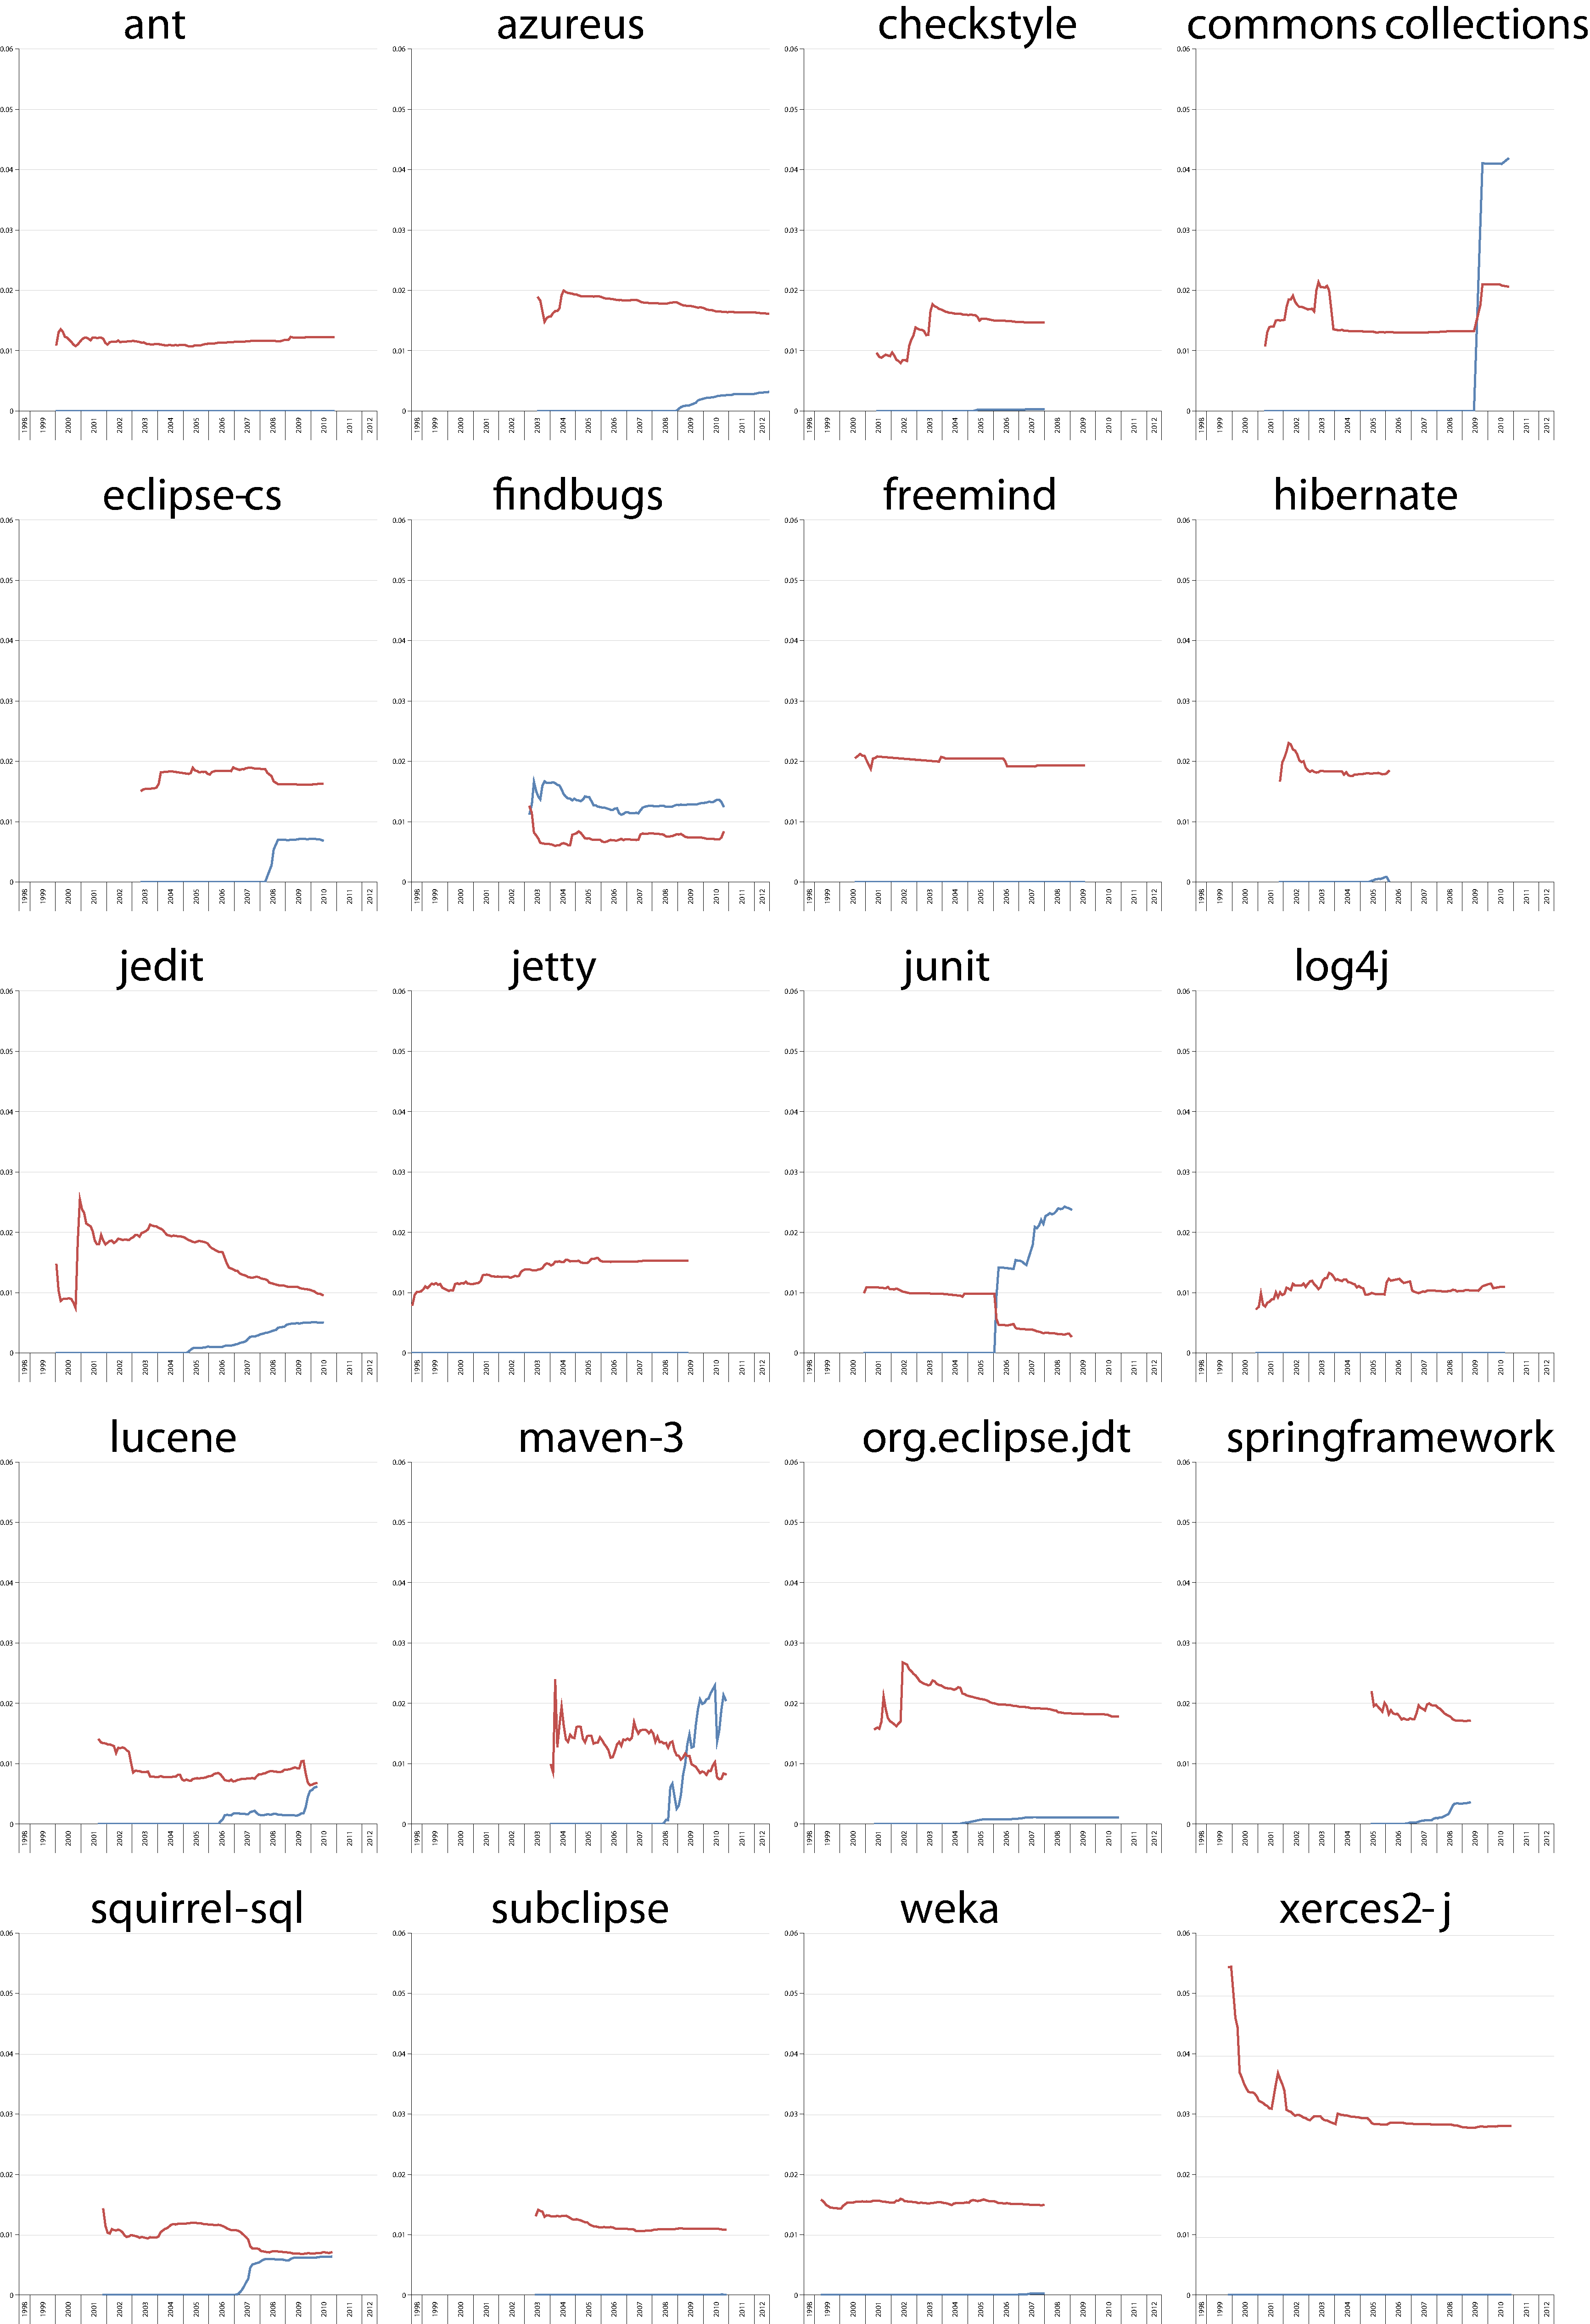
\includegraphics[width=\columnwidth]{cvg-1}
	\caption{Cast versus generic density in established projects.}
\end{figure}

\begin{figure}[htb]
	\centering
	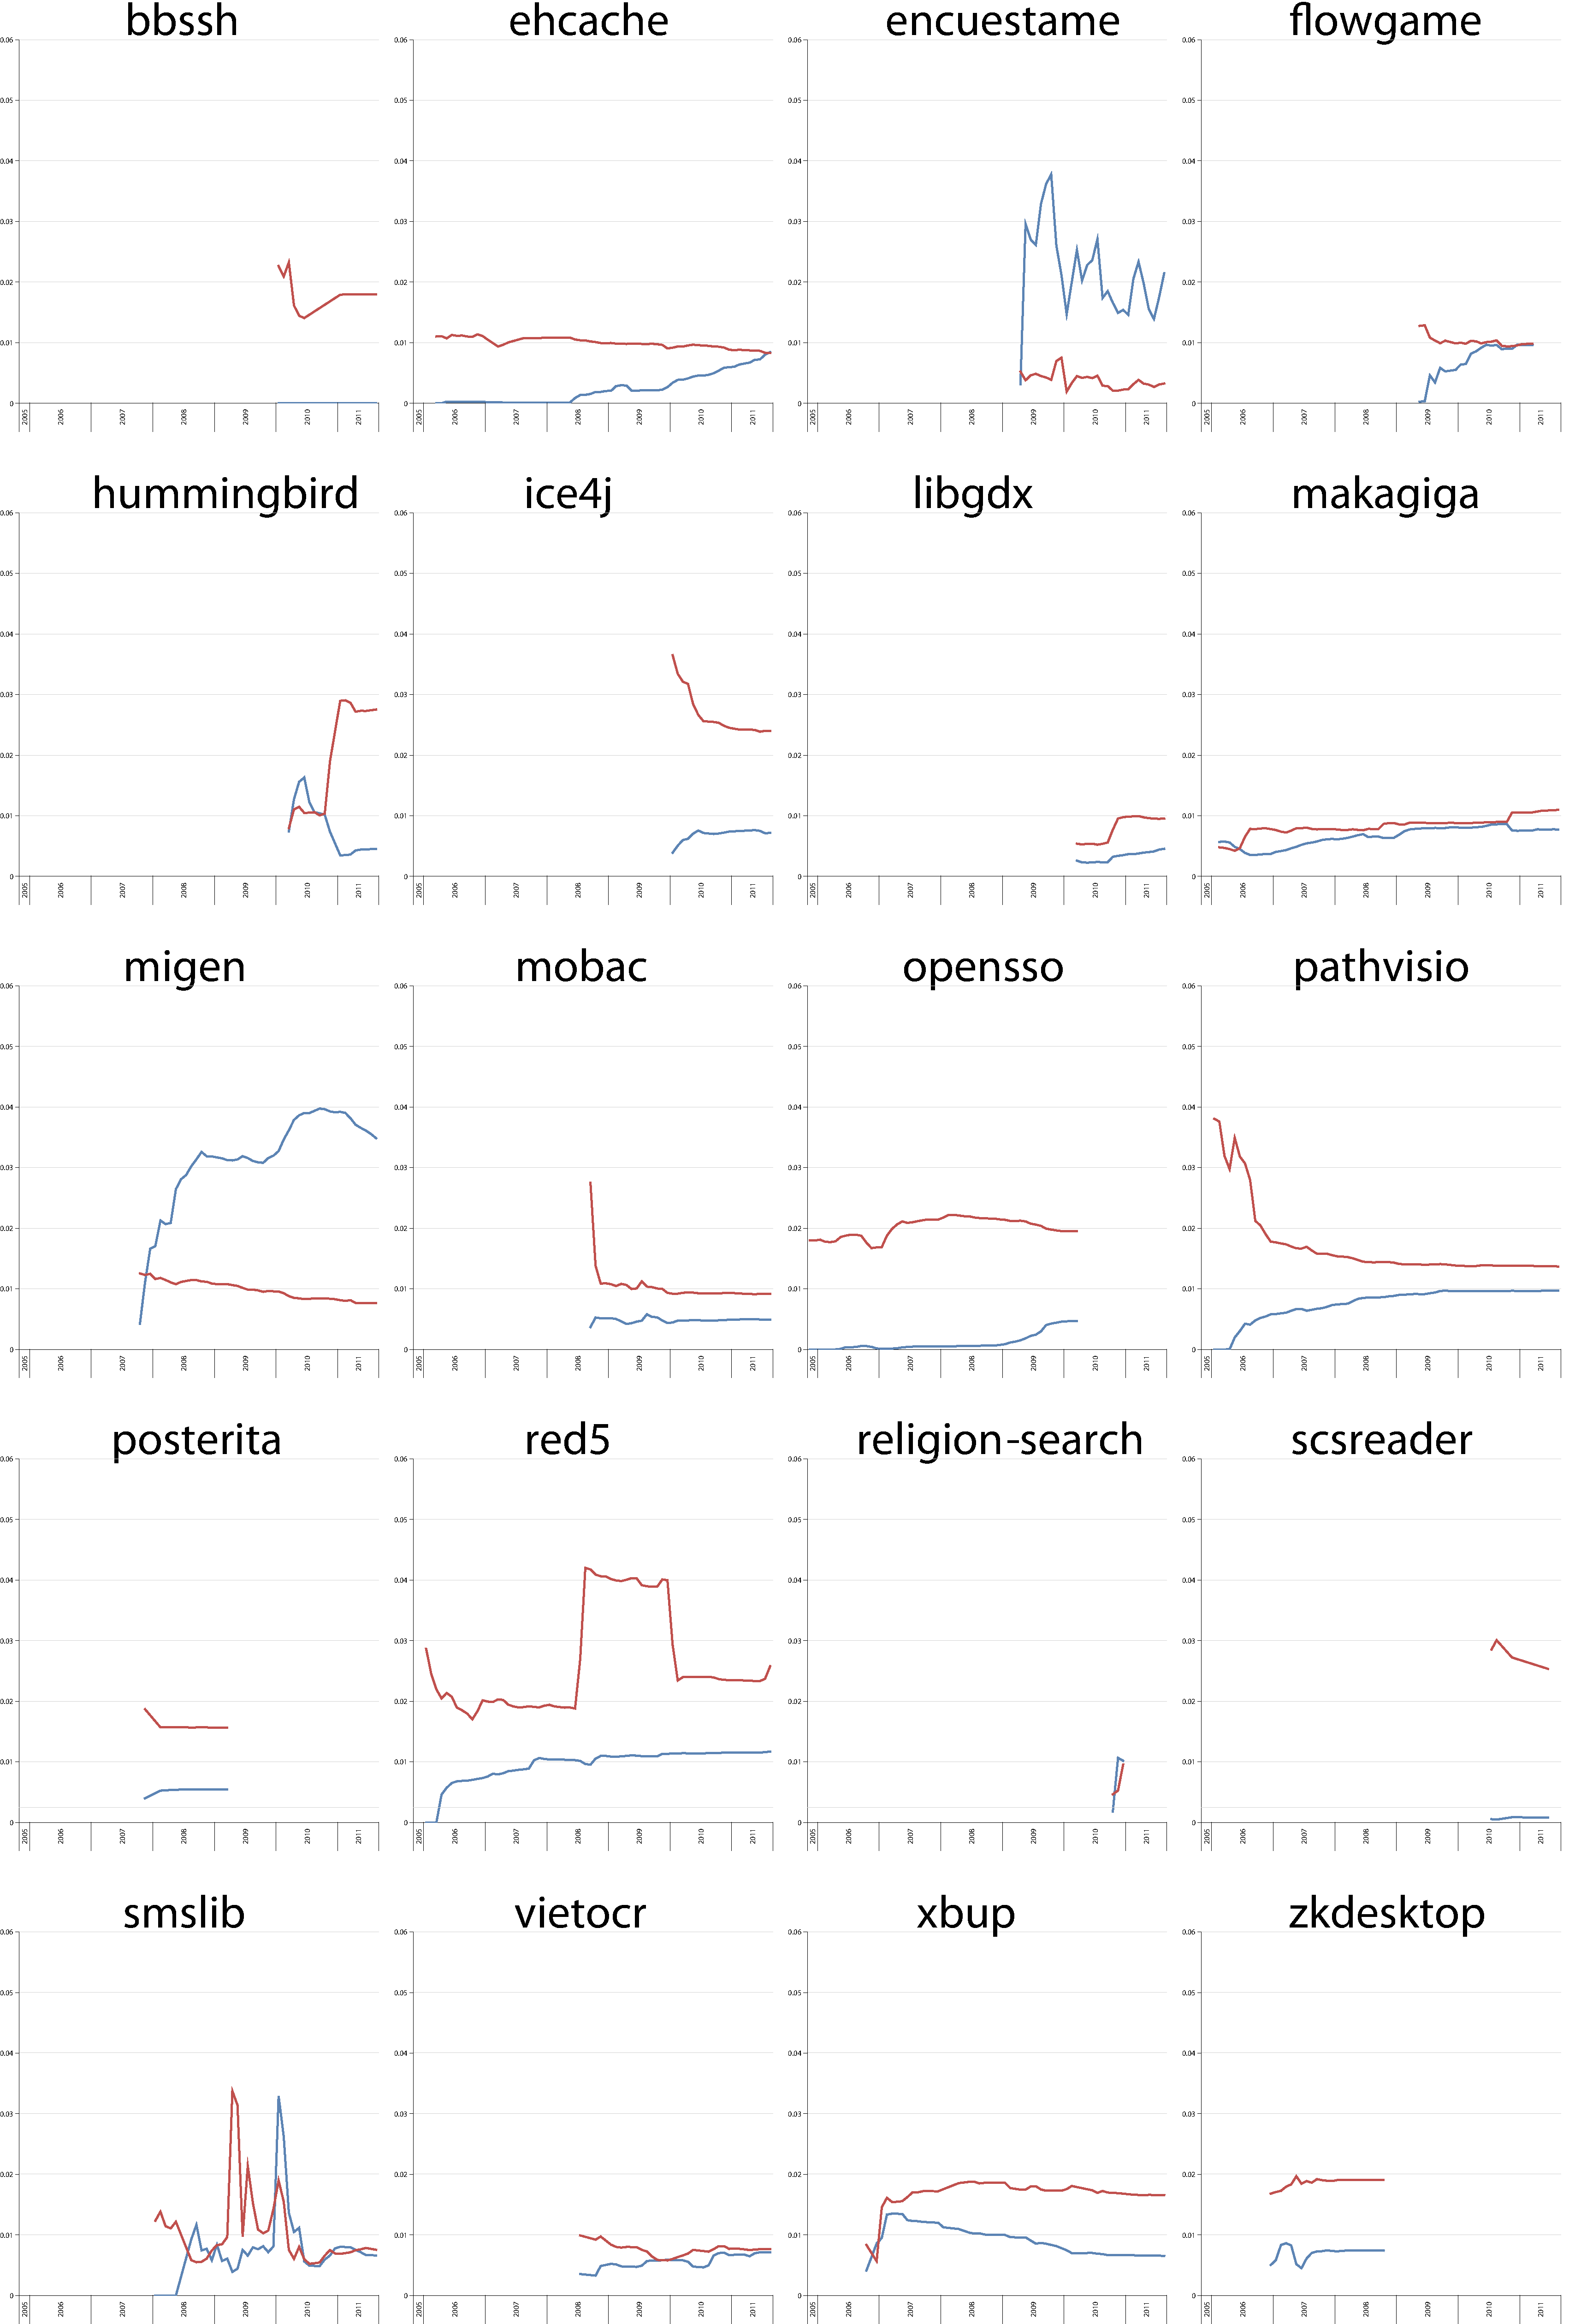
\includegraphics[width=\columnwidth]{cvg-2}
	\caption{Cast versus generic density in recent projects.}
\end{figure}


\newcommand{\tp}[1]{\hspace{-3mm}\includegraphics[width=0.25\columnwidth,page=#1]{types-plots}}
\newcommand{\ap}[1]{\hspace{-3mm}\includegraphics[width=0.25\columnwidth,page=#1]{author-plots}}
\newcommand{\aap}[1]{\hspace{-3mm}\includegraphics[width=0.25\columnwidth,page=#1]{author-annotation-plots}}

\begin{figure}[htb]
	\centering
	\begin{tabular}{cccc}
		\tp{4} & \tp{18} & \tp{11} & \tp{9}\\
		\tp{16} & \tp{15} & \tp{6} & \tp{14}\\
		\tp{5} & \tp{1} & \tp{7} & \tp{8}\\
		\tp{12} & \tp{19} & \tp{10} & \tp{21}\\
		\tp{13} & \tp{17} & \tp{2} & \tp{3}\\	
		%\tp{4} & \tp{18} & \tp{36} & \tp{11}\\
		%\tp{15} & \tp{35} & \tp{6} & \tp{14}\\
		%\tp{7} & \tp{39} & \tp{8} & \tp{12}\\
		%\tp{22} & \tp{10} & \tp{24} & \tp{30}\\
		%\tp{21} & \tp{13} & \tp{17} & \tp{32}\\
	\end{tabular}
	\caption{Usage of raw and generic types in established projects.}
\end{figure}

\begin{figure}[htb]
	\centering
	\begin{tabular}{cccc}
		\tp{36} & \tp{26} & \tp{34} & \tp{35}\\
		\tp{38} & \tp{37} & \tp{39} & \tp{25}\\
		\tp{29} & \tp{33} & \tp{22} & \tp{24}\\
		\tp{30} & \tp{23} & \tp{41} & \tp{40}\\
		\tp{31} & \tp{32} & \tp{27} & \tp{28}\\
		%\tp{9} & \tp{16} & \tp{26} & \tp{34}\\
		%\tp{38} & \tp{37} & \tp{5} & \tp{1}\\
		%\tp{25} & \tp{19} & \tp{29} & \tp{33}\\
		%\tp{23} & \tp{41} & \tp{40} & \tp{31}\\
		%\tp{2} & \tp{27} & \tp{3} & \tp{28}\\
	\end{tabular}
	\caption{Usage of raw and generic types in recent projects.}
\end{figure}

\begin{figure}[htb]
	\centering
	\begin{tabular}{cccc}
		\ap{4} & \ap{18} & \ap{11} & \ap{9}\\
		\ap{16} & \ap{10} & \ap{15} & \ap{6}\\
		\ap{14} & \ap{5} & \ap{1} & \ap{7}\\
		\ap{8} & \ap{12} & \ap{19} & \ap{21}\\
		\ap{13} & \ap{17} & \ap{2} & \ap{3}\\	
		%\ap{4} & \ap{18} & \ap{36} & \ap{11}\\
		%\ap{15} & \ap{35} & \ap{6} & \ap{14}\\
		%\ap{7} & \ap{39} & \ap{8} & \ap{12}\\
		%\ap{22} & \ap{10} & \ap{24} & \ap{30}\\
		%\ap{21} & \ap{13} & \ap{17} & \ap{32}\\
	\end{tabular}
	\caption{Contributors' introduction and removal of parameterized types over time in established projects.}
\end{figure}

\begin{figure}[htb]
	\centering
	\begin{tabular}{cccc}
		\ap{36} & \ap{26} & \ap{34} & \ap{35}\\
		\ap{38} & \ap{37} & \ap{39} & \ap{25}\\
		\ap{29} & \ap{33} & \ap{22} & \ap{24}\\
		\ap{30} & \ap{23} & \ap{41} & \ap{40}\\
		\ap{31} & \ap{32} & \ap{27} & \ap{28}\\
		%\ap{9} & \ap{16} & \ap{26} & \ap{34}\\
		%\ap{38} & \ap{37} & \ap{5} & \ap{1}\\
		%\ap{25} & \ap{19} & \ap{29} & \ap{33}\\
		%\ap{23} & \ap{41} & \ap{40} & \ap{31}\\
		%\ap{2} & \ap{27} & \ap{3} & \ap{28}\\
	\end{tabular}
	\caption{Contributors' introduction and removal of parameterized types over time in recent projects.}
\end{figure}

\begin{figure}[htb]
	\centering
	\begin{tabular}{cccc}
		\aap{4} & \aap{18} & \aap{11} & \aap{9}\\
		\aap{16} & \aap{10} & \aap{15} & \aap{6}\\
		\aap{14} & \aap{5} & \aap{1} & \aap{7}\\
		\aap{8} & \aap{12} & \aap{19} & \aap{21}\\
		\aap{13} & \aap{17} & \aap{2} & \aap{3}\\	
		%\aap{4} & \aap{18} & \aap{36} & \aap{11}\\
		%\aap{15} & \aap{35} & \aap{6} & \aap{14}\\
		%\aap{7} & \aap{39} & \aap{8} & \aap{12}\\
		%\aap{22} & \aap{10} & \aap{24} & \aap{30}\\
		%\aap{21} & \aap{13} & \aap{17} & \aap{32}\\
	\end{tabular}
	\caption{Contributors' introduction and removal of annotations over time in established projects.}
\end{figure}

\begin{figure}[htb]
	\centering
	\begin{tabular}{cccc}
		\aap{36} & \aap{26} & \aap{34} & \aap{35}\\
		\aap{38} & \aap{37} & \aap{39} & \aap{25}\\
		\aap{29} & \aap{33} & \aap{22} & \aap{24}\\
		\aap{30} & \aap{23} & \aap{41} & \aap{40}\\
		\aap{31} & \aap{32} & \aap{27} & \aap{28}\\
		%\aap{9} & \aap{16} & \aap{26} & \aap{34}\\
		%\aap{38} & \aap{37} & \aap{5} & \aap{1}\\
		%\aap{25} & \aap{19} & \aap{29} & \aap{33}\\
		%\aap{23} & \aap{41} & \aap{40} & \aap{31}\\
		%\aap{2} & \aap{27} & \aap{3} & \aap{28}\\
	\end{tabular}
	\caption{Contributors' introduction and removal of annotations over time in recent projects.}
\end{figure}



%%%%% MOVED OUT
%\subsection{Related work}

%Kiezun~\etal~\cite{kiezun2007refactoring} focus on parameterizing Java classes.
%They discuss the two problems faced by developers in using generics and
%the process of generification.

%\begin{enumerate}

%\item The \emph{parameterization problem} consists of adding type parameters to
%an existing class definition so that it can be used in different contexts
%without the loss of type information.

%\item Once a class has been parameterized, the \emph{instantiation problem} is
%the task of determining the type arguments that should be passed to instances of
%the generic class in client code.

%\end{enumerate}

%\noindent
%In this paper we address both problems by examining both class and method
%\emph{parameterization} and \emph{instantiation}.
%Through personal communication, Kiezun found that when the Java Collections
%Framework was parameterized manually, the developers involved with the task
%described it as very time consuming, tedious, and error prone.

%In a paper on the design and implementation of .NET at Microsoft, Kennedy and
%Syme~\cite{kennedy2001design} describe their design decisions when they added
%generics to .NET.  At the beginning of the paper, they list the advantages of
%generics over dynamically typed languages.

%\begin{enumerate}
%\item Safety - more bugs caught at compile time
%\item Expressivity - more invariants expressed in type signatures
%\item Clarity - fewer explicit conversions between data types
%\item Efficiency - no need for run-time type checks
%\end{enumerate}

\end{document}




